\documentclass[10pt]{beamer}
\usefonttheme{professionalfonts,serif}
\def\newblock{\hskip .11em plus .33em minus .07em}
\usepackage[numbers,sort]{natbib}
\renewcommand{\rmdefault}{psbx}
\usepackage[utf8]{inputenc}
\usepackage[T1]{fontenc}
\usepackage{textcomp}
\usepackage{eulervm}

\usetheme{default}           % tips from David Blei
\useinnertheme{circles}
\useoutertheme{infolines}
\setbeamertemplate{headline}{}
\setbeamertemplate{navigation symbols}{}
\setbeamerfont{itemize/enumerate subbody}{size=\normalsize}
\setbeamerfont{itemize/enumerate subsubbody}{size=\normalsize}
\usecolortheme{seahorse}
\setbeamersize{text margin left=2mm,text margin right=2mm}

\graphicspath{{../../figures/}}

\definecolor{mypine}{rgb}{0.05,0.45,0.05}
\definecolor{mycyan}{rgb}{0.0,0.9,0.9}
\newcommand{\Red}{\textcolor{red}}
\newcommand{\Blue}{\textcolor{blue}}
\newcommand{\Green}{\textcolor{mypine}}
\newcommand{\PineGreen}{\textcolor{mypine}}
\newcommand{\Magenta}{\textcolor{magenta}}
\newcommand{\Cyan}{\textcolor{mycyan}}

\newcommand{\N}{\mathcal{N}}
\newcommand{\R}{\mathbb{R}}
\newcommand{\T}{{\scriptsize^{\top}}}
\newcommand{\D}{\mathcal{D}}
\newcommand{\F}{\mathcal{F}}
\newcommand{\E}{\mathbb{E}}
\newcommand{\V}{\mathbb{V}}
\newcommand{\M}{\mathcal{M}}
\newcommand{\KL}{\mathcal{KL}}
\newcommand{\cut}[1]{}
\newcommand{\trace}{\operatorname{trace}}

\newcommand{\bmu}{{\boldsymbol{\mu}}}
\newcommand{\btheta}{\boldsymbol{\theta}}
\newcommand{\bepsilon}{\boldsymbol{\epsilon}}
\newcommand{\balpha}{\boldsymbol{\alpha}}
\newcommand{\bbeta}{\boldsymbol{\beta}}
\newcommand{\bphi}{\boldsymbol{\phi}}
\newcommand{\bPhi}{\boldsymbol{\Phi}}
\newcommand{\bSigma}{\boldsymbol{\Sigma}}
\newcommand{\bpi}{\boldsymbol{\pi}}
\newcommand{\blambda}{\boldsymbol{\lambda}}

\newcommand{\argmax}{\operatorname{argmax}}
\newcommand{\argmin}{\operatorname{argmin}}
\newcommand{\ci}{{\bot\negthickspace\negthickspace\bot}} % conditional indep.
\newcommand{\neigh}{\operatorname{ne}}
\newcommand{\vectr}[2]{  \left[ \!\!\begin{array}{c} #1 \\
      #2 \end{array} \!\!\right]}
\newcommand{\deff}{\stackrel{\mathrm{def}}{=}}
\newcommand{\deldel}[2]{\frac{\partial #1}{\partial #2}}

\newcommand{\maketilde}{\raisebox{0.4ex}{\tiny $\sim$}}
\newcommand{\bfa}{\mathbf a}
\newcommand{\bfb}{\mathbf b}
\newcommand{\bfe}{\mathbf e}
\newcommand{\bff}{\mathbf f}
\newcommand{\bfk}{\mathbf k}
\newcommand{\bfm}{\mathbf m}
\newcommand{\bfn}{\mathbf n}
\newcommand{\bfp}{\mathbf{p}}
\newcommand{\bfs}{\mathbf s}
\newcommand{\bfu}{\mathbf u}
\newcommand{\bfx}{\mathbf x}
\newcommand{\bfy}{\mathbf y}
\newcommand{\bft}{\mathbf t}
\newcommand{\bfv}{\mathbf v}
\newcommand{\bfw}{\mathbf w}
\newcommand{\bfA}{\mathbf A}
\newcommand{\bfI}{\mathbf I}
\newcommand{\bfK}{\mathbf K}


\title{Finite and infinite basis GPs}
\author{Carl Edward Rasmussen}
\date{October 13th, 2016}

\begin{document}

\begin{frame}
\titlepage
\end{frame}

\begin{frame}
\frametitle{From infinite linear models to Gaussian processes}

Consider the class of functions (sums of squared exponentials):
\[
\begin{split}
f(x)\;=&\;\lim_{N\rightarrow\infty}\frac{1}{N}\sum_{n=-N/2}^{N/2}\gamma_n\exp(-(x-\tfrac{n}{\sqrt{N}})^2),
\text{\ \ where\ \ }\gamma_n\sim{\cal N}
(0, 1),\;\forall n\\
=&\;\int_{-\infty}^\infty\!\! \gamma(u)\exp(-(x-u)^2)du,
\text{\ \ where\ \ }\gamma(u)\sim{\cal N}(0,1),\;\forall u.
\end{split}
\]
The mean function is:
\[
\mu(x)\;=\;E[f(x)]\;=\;\int_{-\infty}^\infty\exp(-(x-u)^2)
\int_{-\infty}^\infty\!\!\gamma(u) p(\gamma(u))d\gamma(u) \; \; du\;=\;0,
\]
and the covariance function:
\[
\begin{split}
E&[f(x)f(x')]\;=\;\int\exp\big(\!-(x-u)^2-(x'-u)^2\big)du\\
=&\;\int\exp\big(\!-2(u-\frac{x+x'}{2})^2+\frac{(x+x')^2}{2}-x^2-x'^2\big)du
\;\propto\;\exp\big(\!-\frac{(x-x')^2}{2}\big).
\end{split}
\]
Thus, the squared exponential covariance function is equivalent to regression
using infinitely many Gaussian shaped basis functions placed everywhere,
\Red{not just at your training points!}
\end{frame}


\begin{frame}
\frametitle{\!\!\!Using finitely many basis functions may be dangerous!(1)}

Finite linear model with 5 localized basis functions)

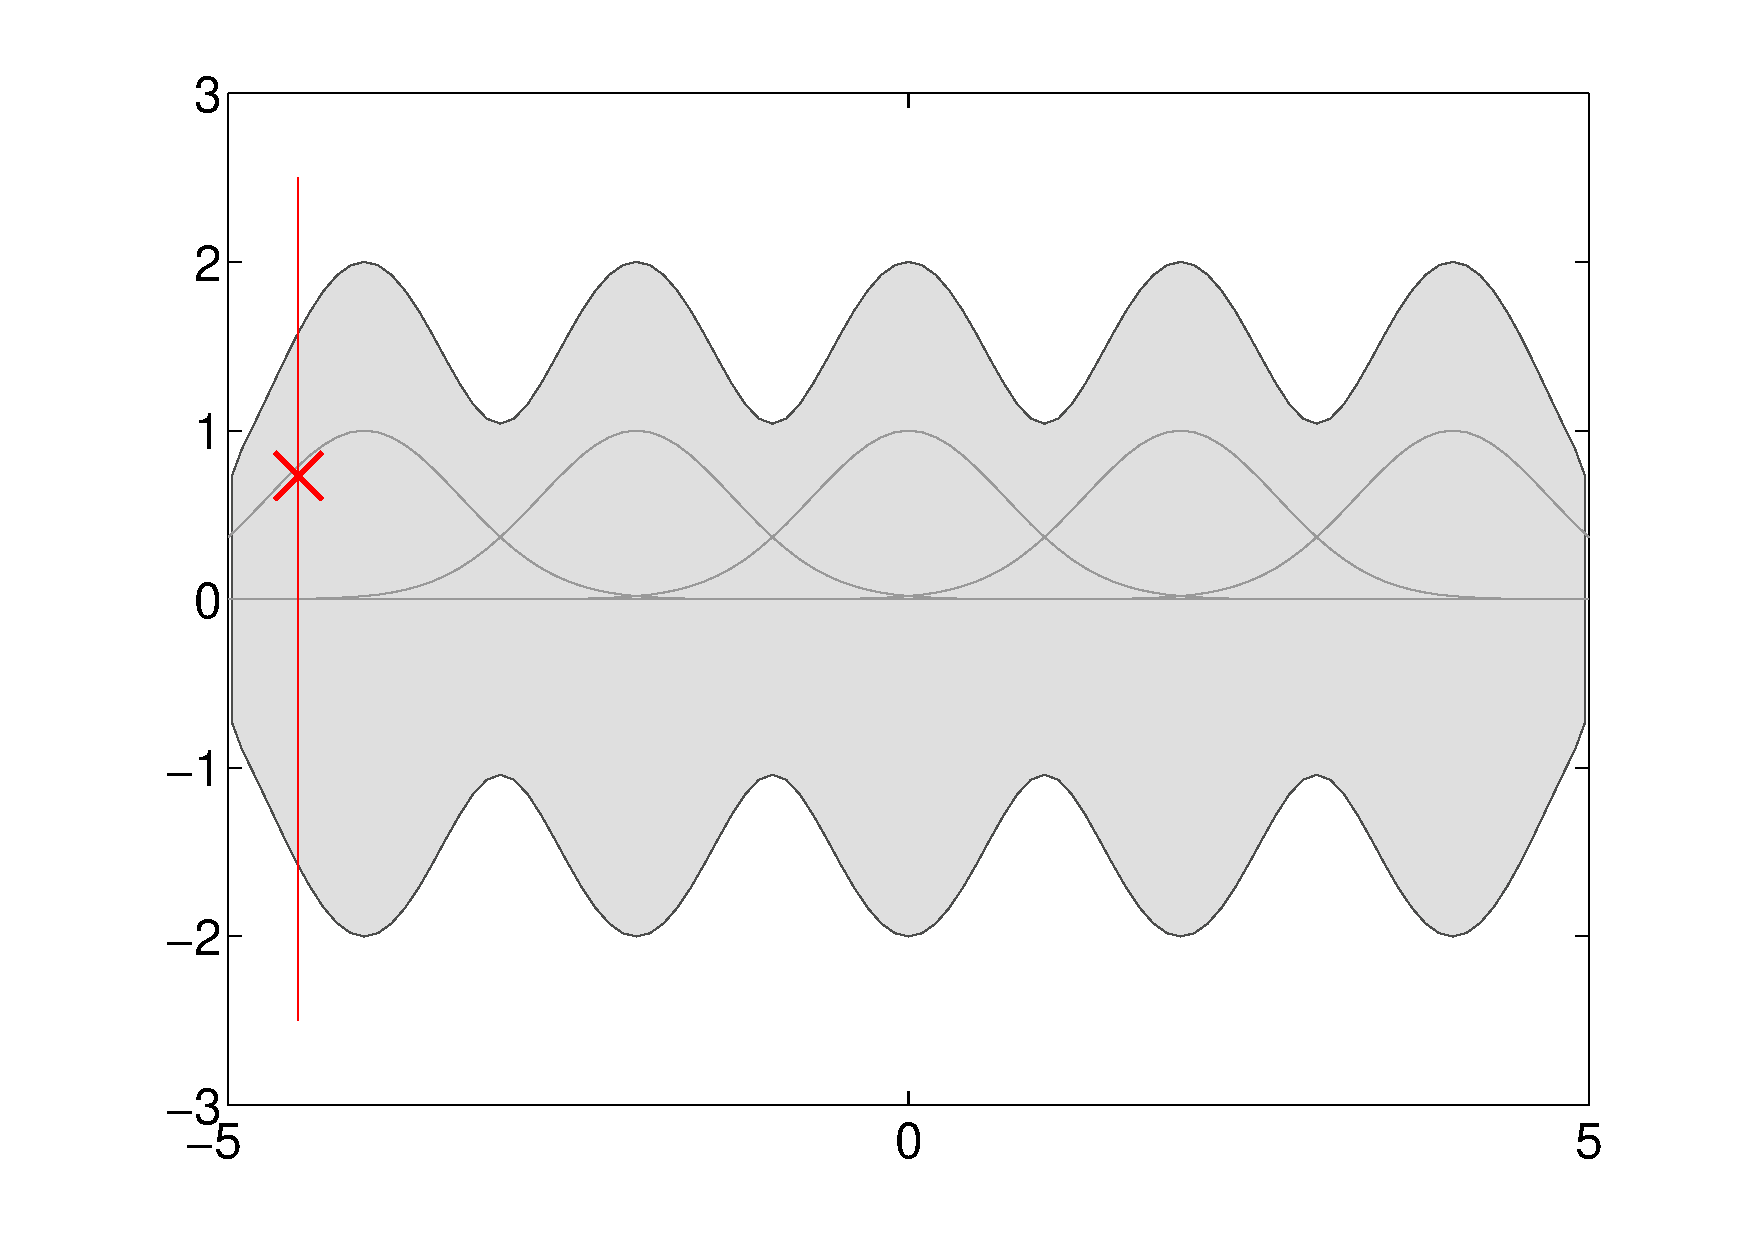
\includegraphics[width=0.33\textwidth]{seq_linear_M1.pdf}
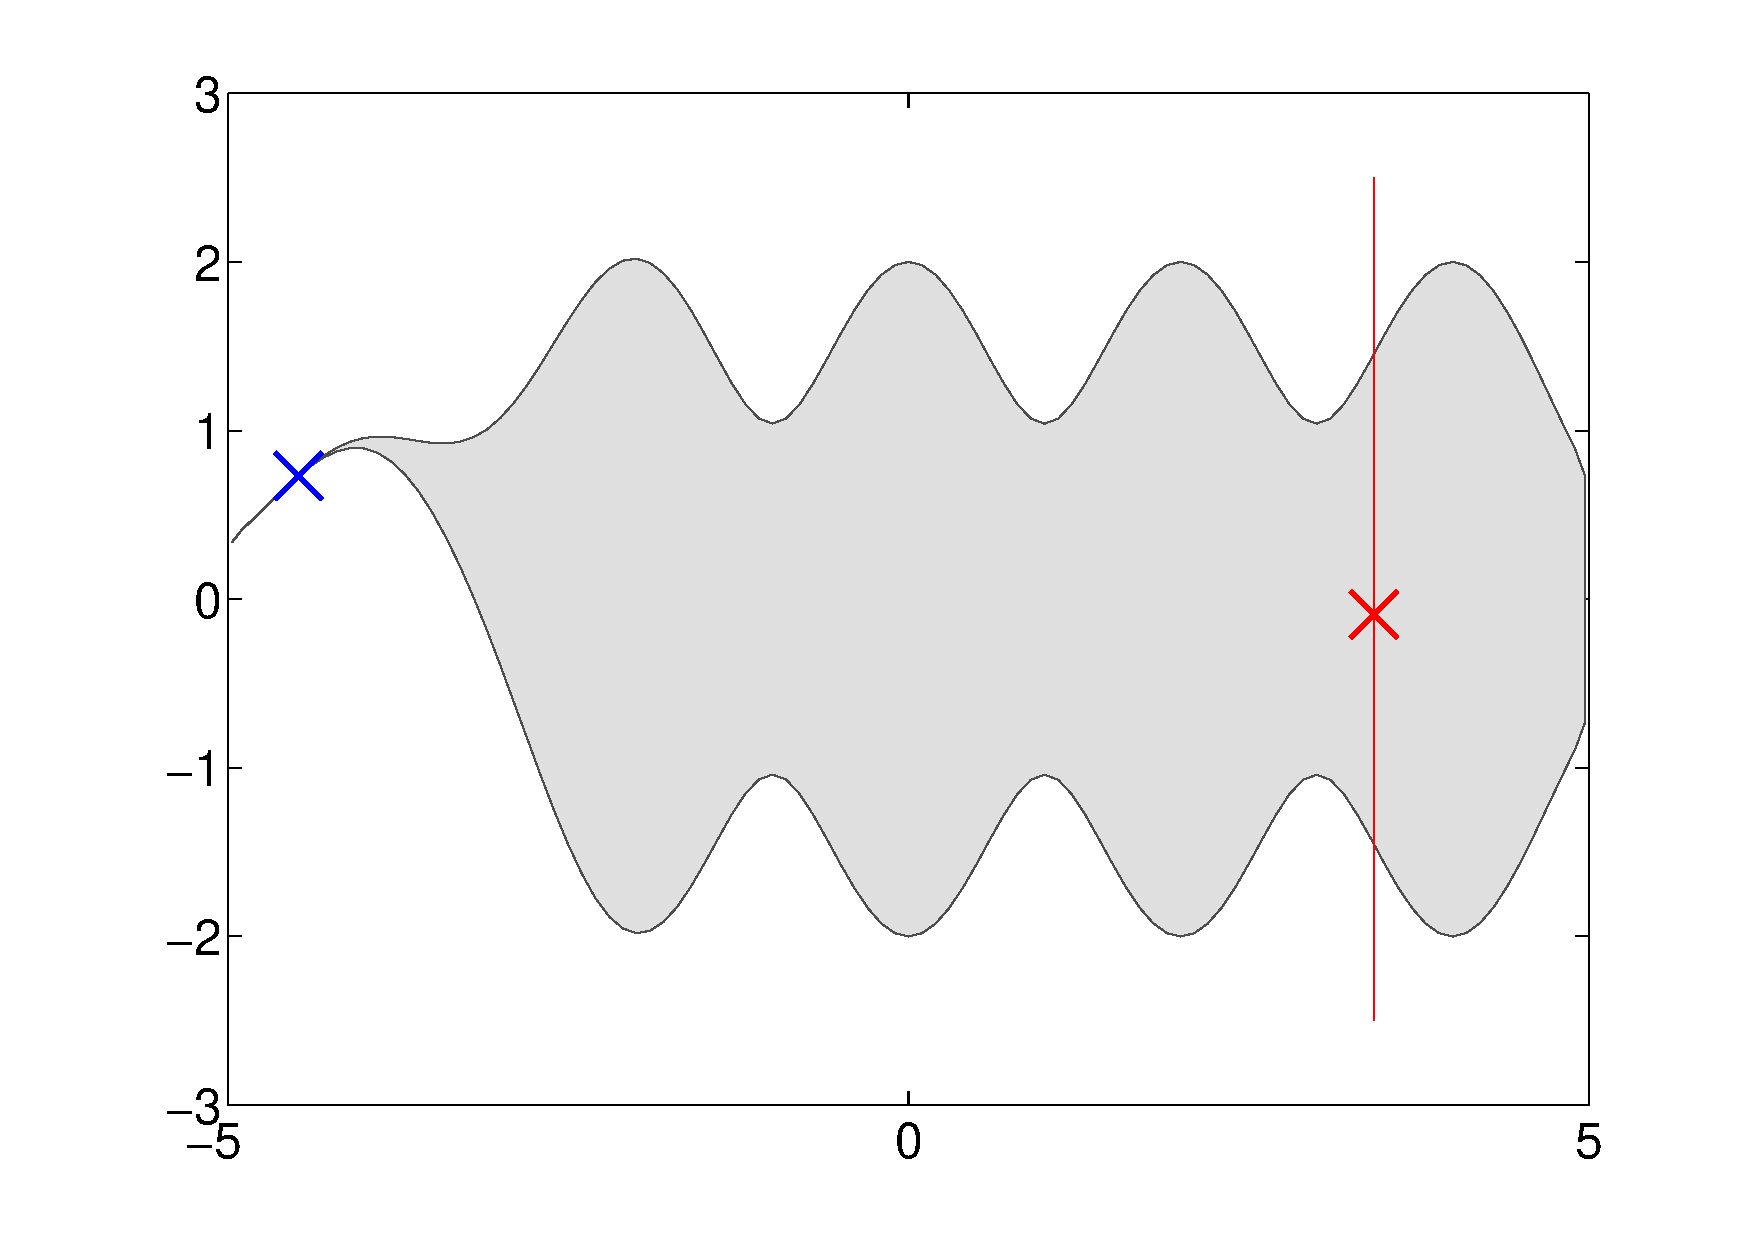
\includegraphics[width=0.33\textwidth]{seq_linear_M2.pdf}
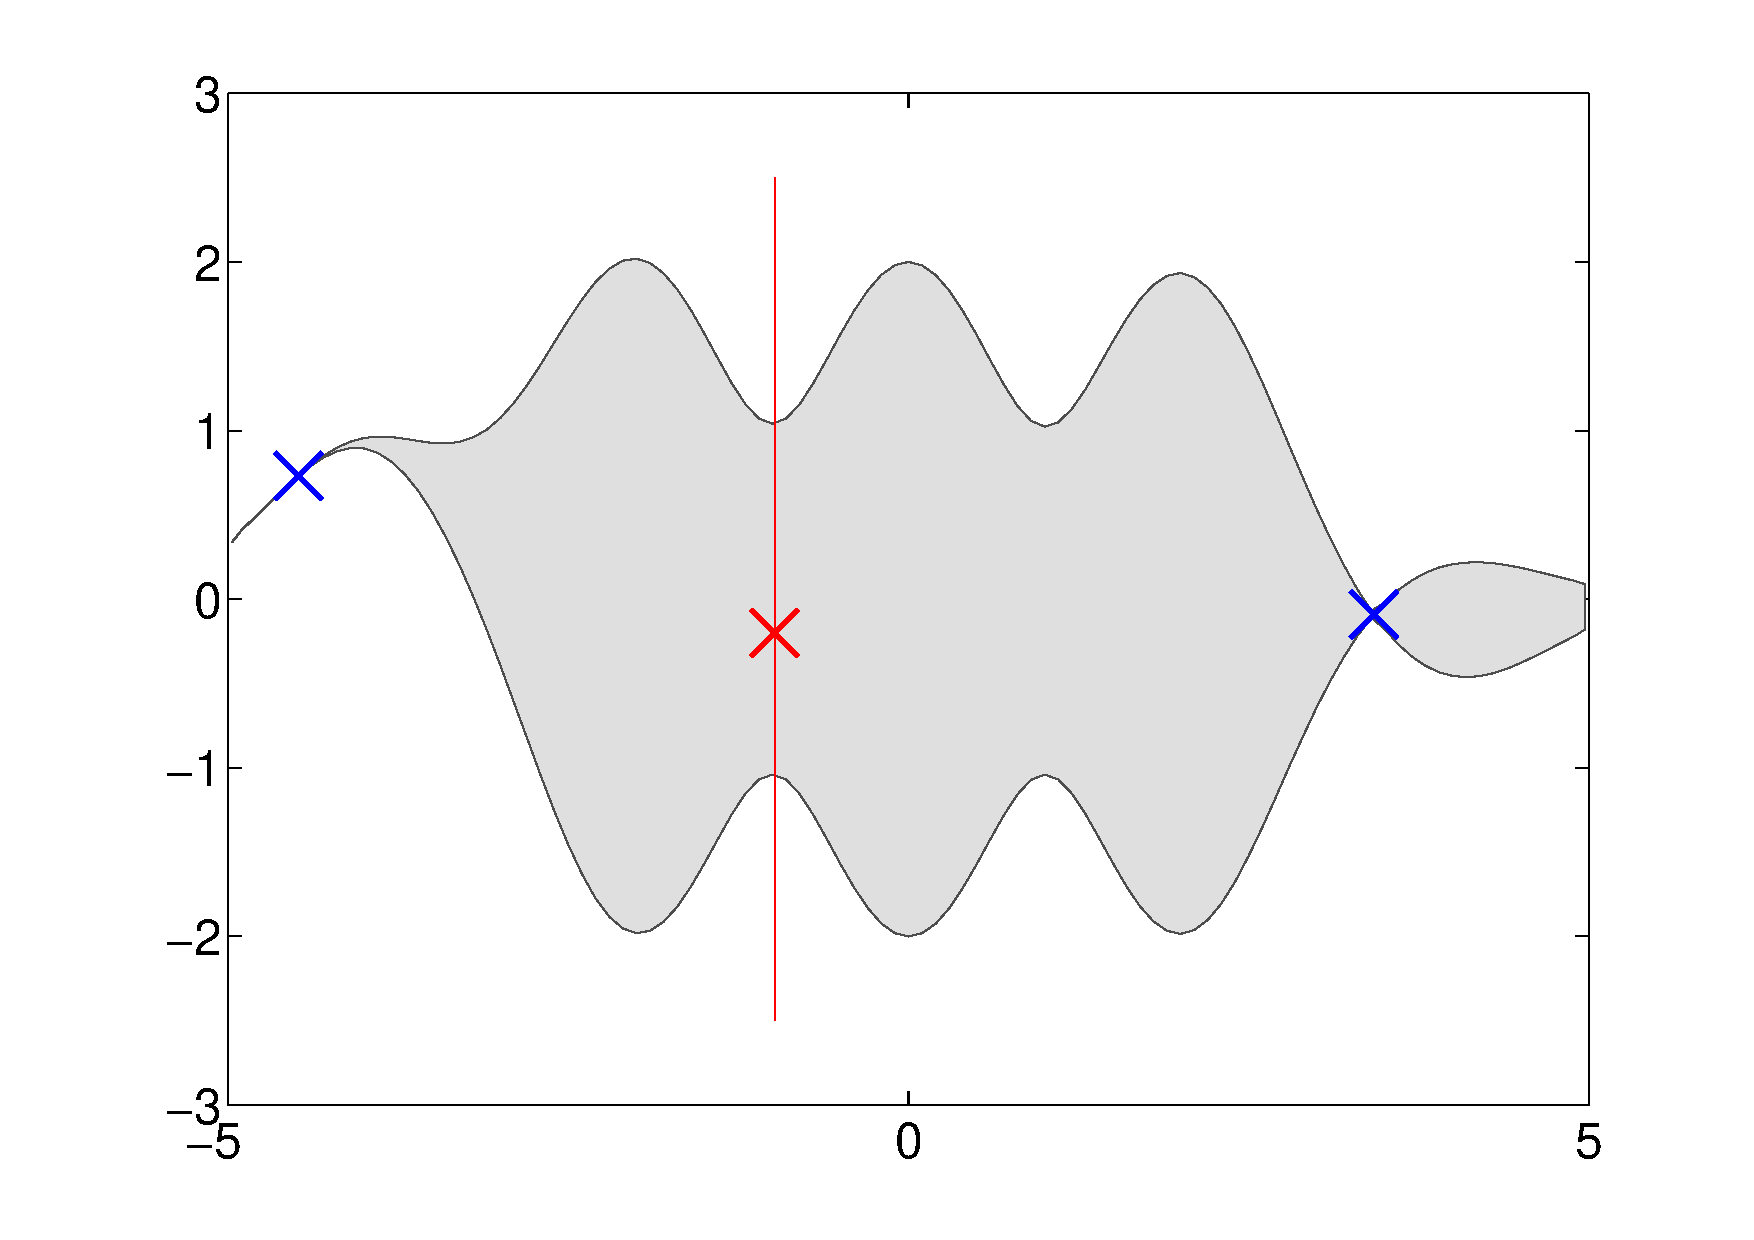
\includegraphics[width=0.33\textwidth]{seq_linear_M3.pdf}

Gaussian process with infinitely many localized basis functions
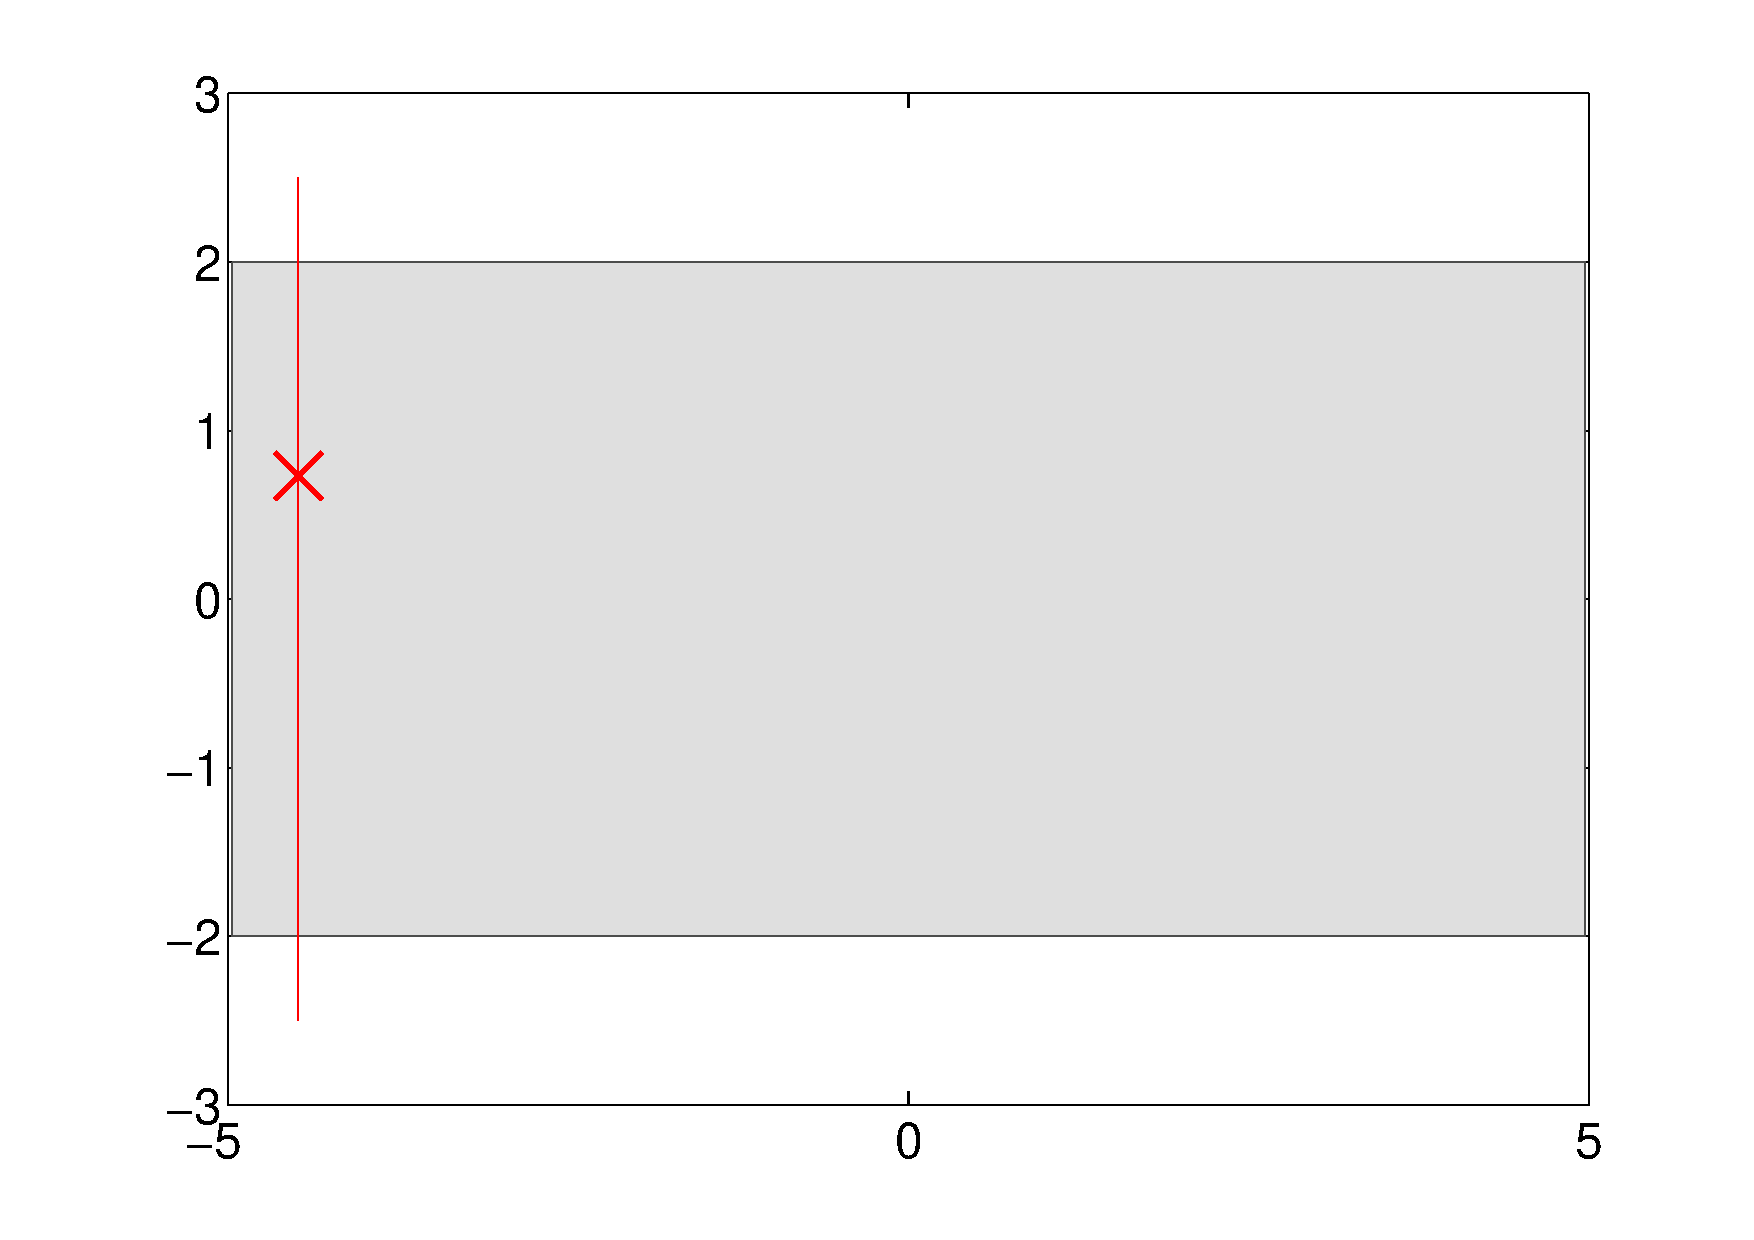
\includegraphics[width=0.33\textwidth]{seq_fullGP_M1.pdf}
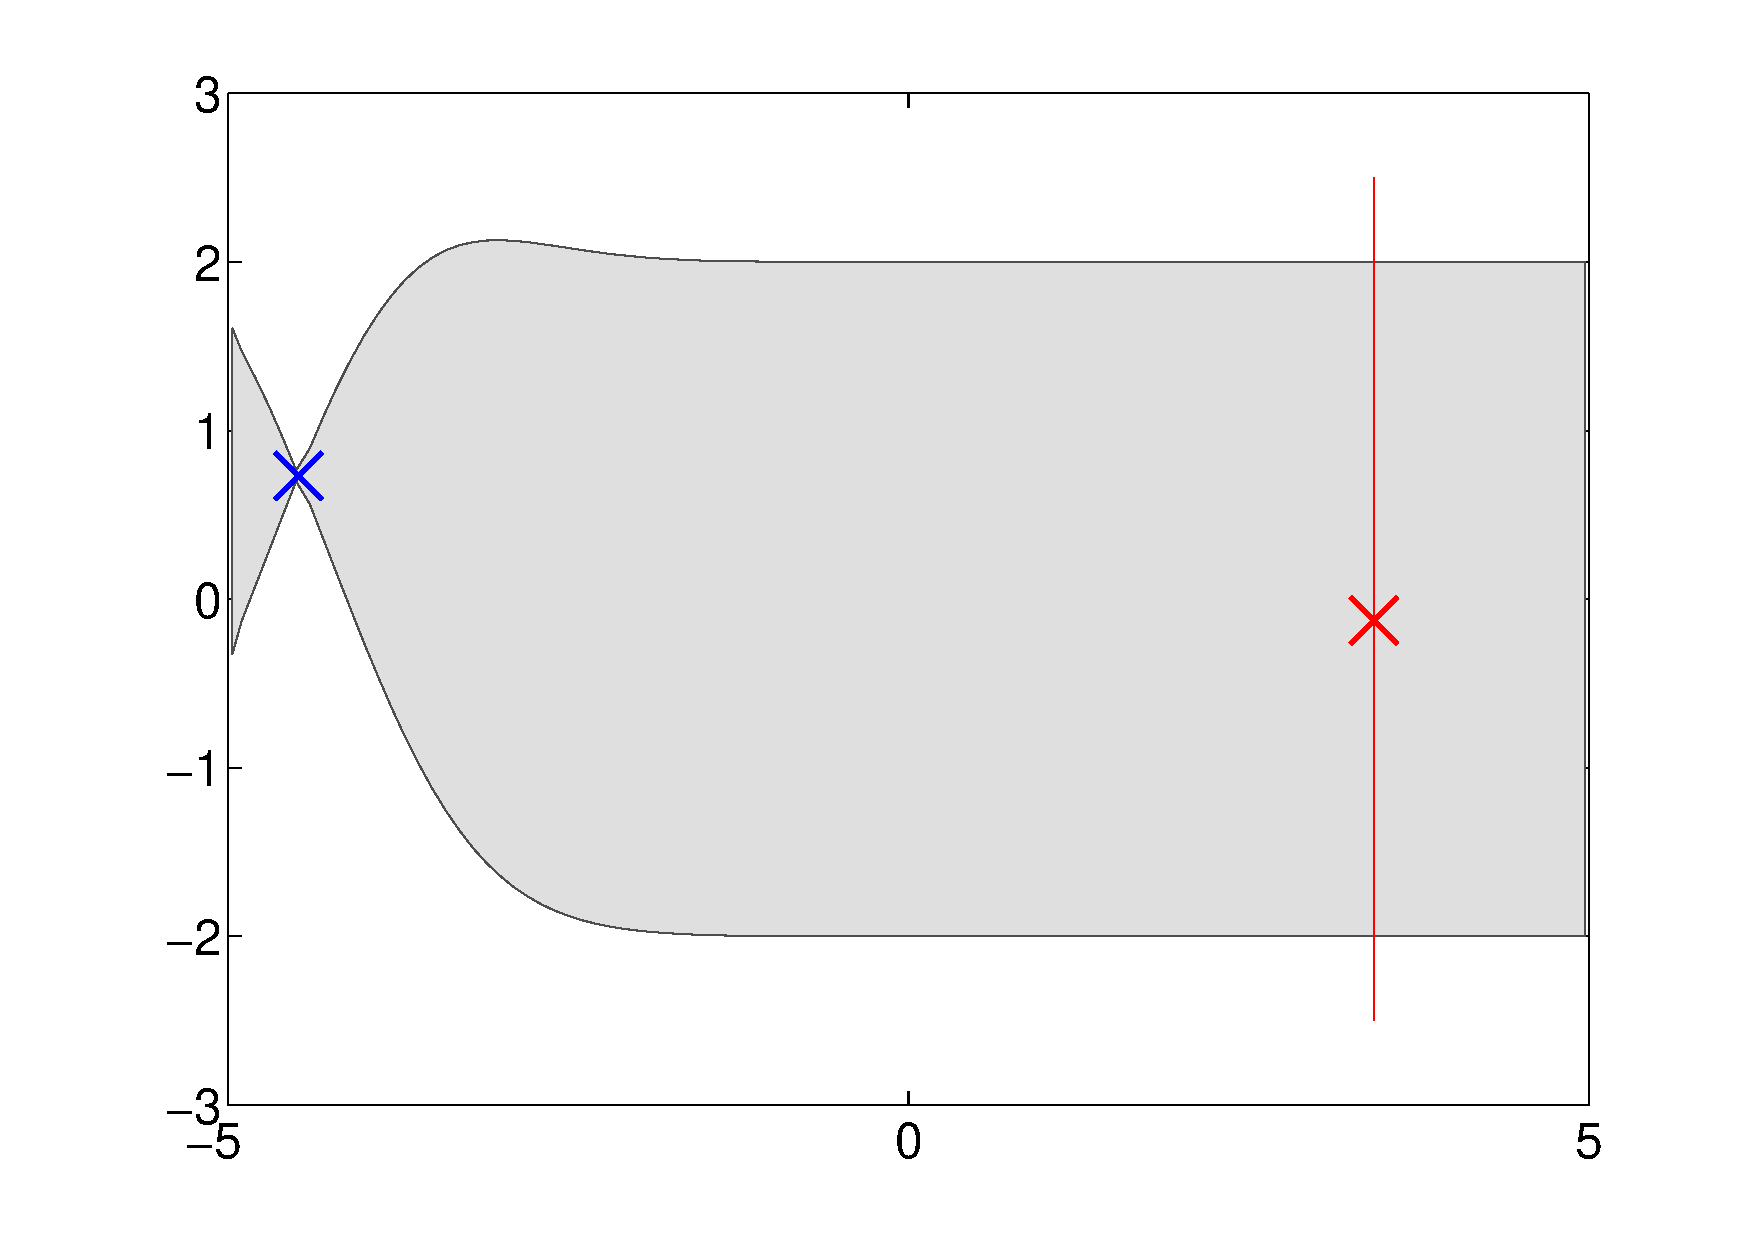
\includegraphics[width=0.33\textwidth]{seq_fullGP_M2.pdf}
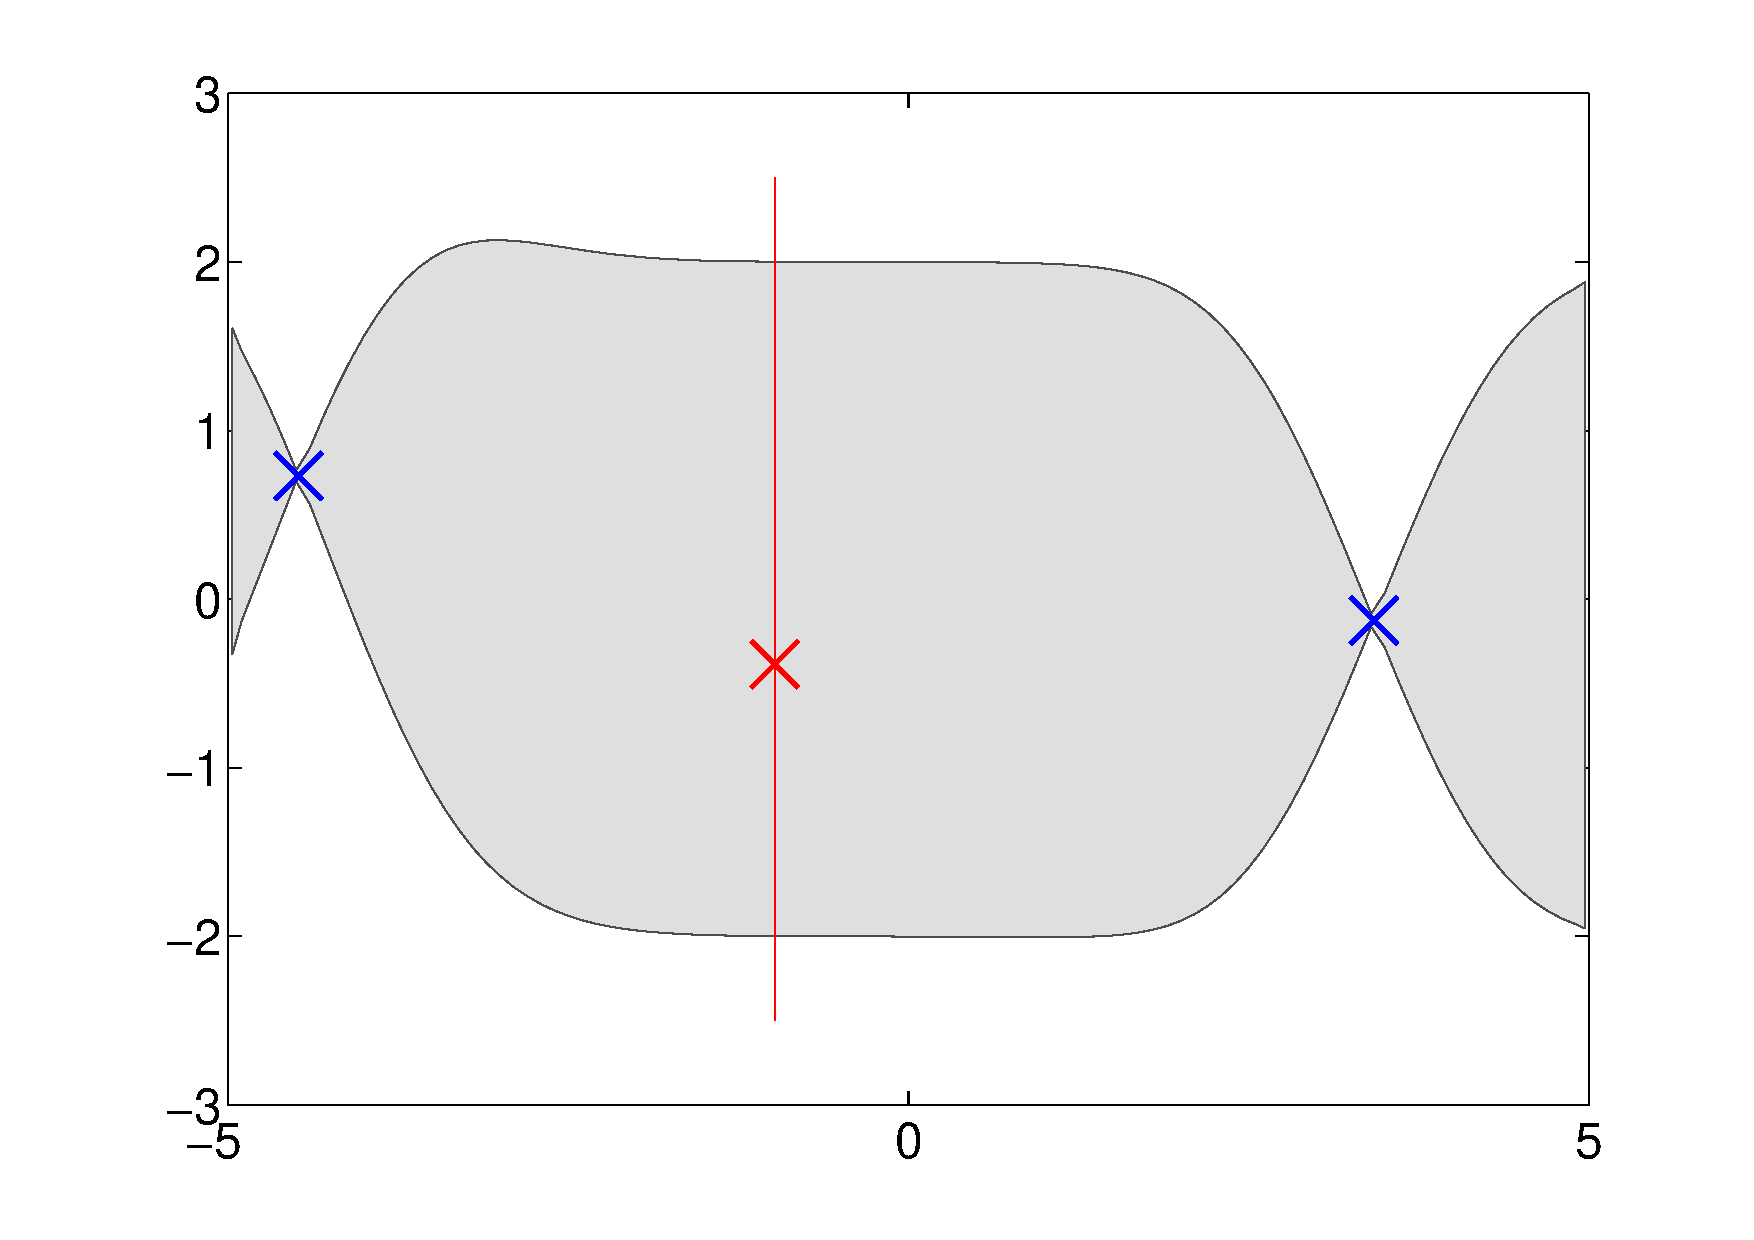
\includegraphics[width=0.33\textwidth]{seq_fullGP_M3.pdf}


\end{frame}

\begin{frame}
\frametitle{\!\!\!Using finitely many basis functions may be dangerous!(2)}

Finite linear model with 5 localized basis functions)

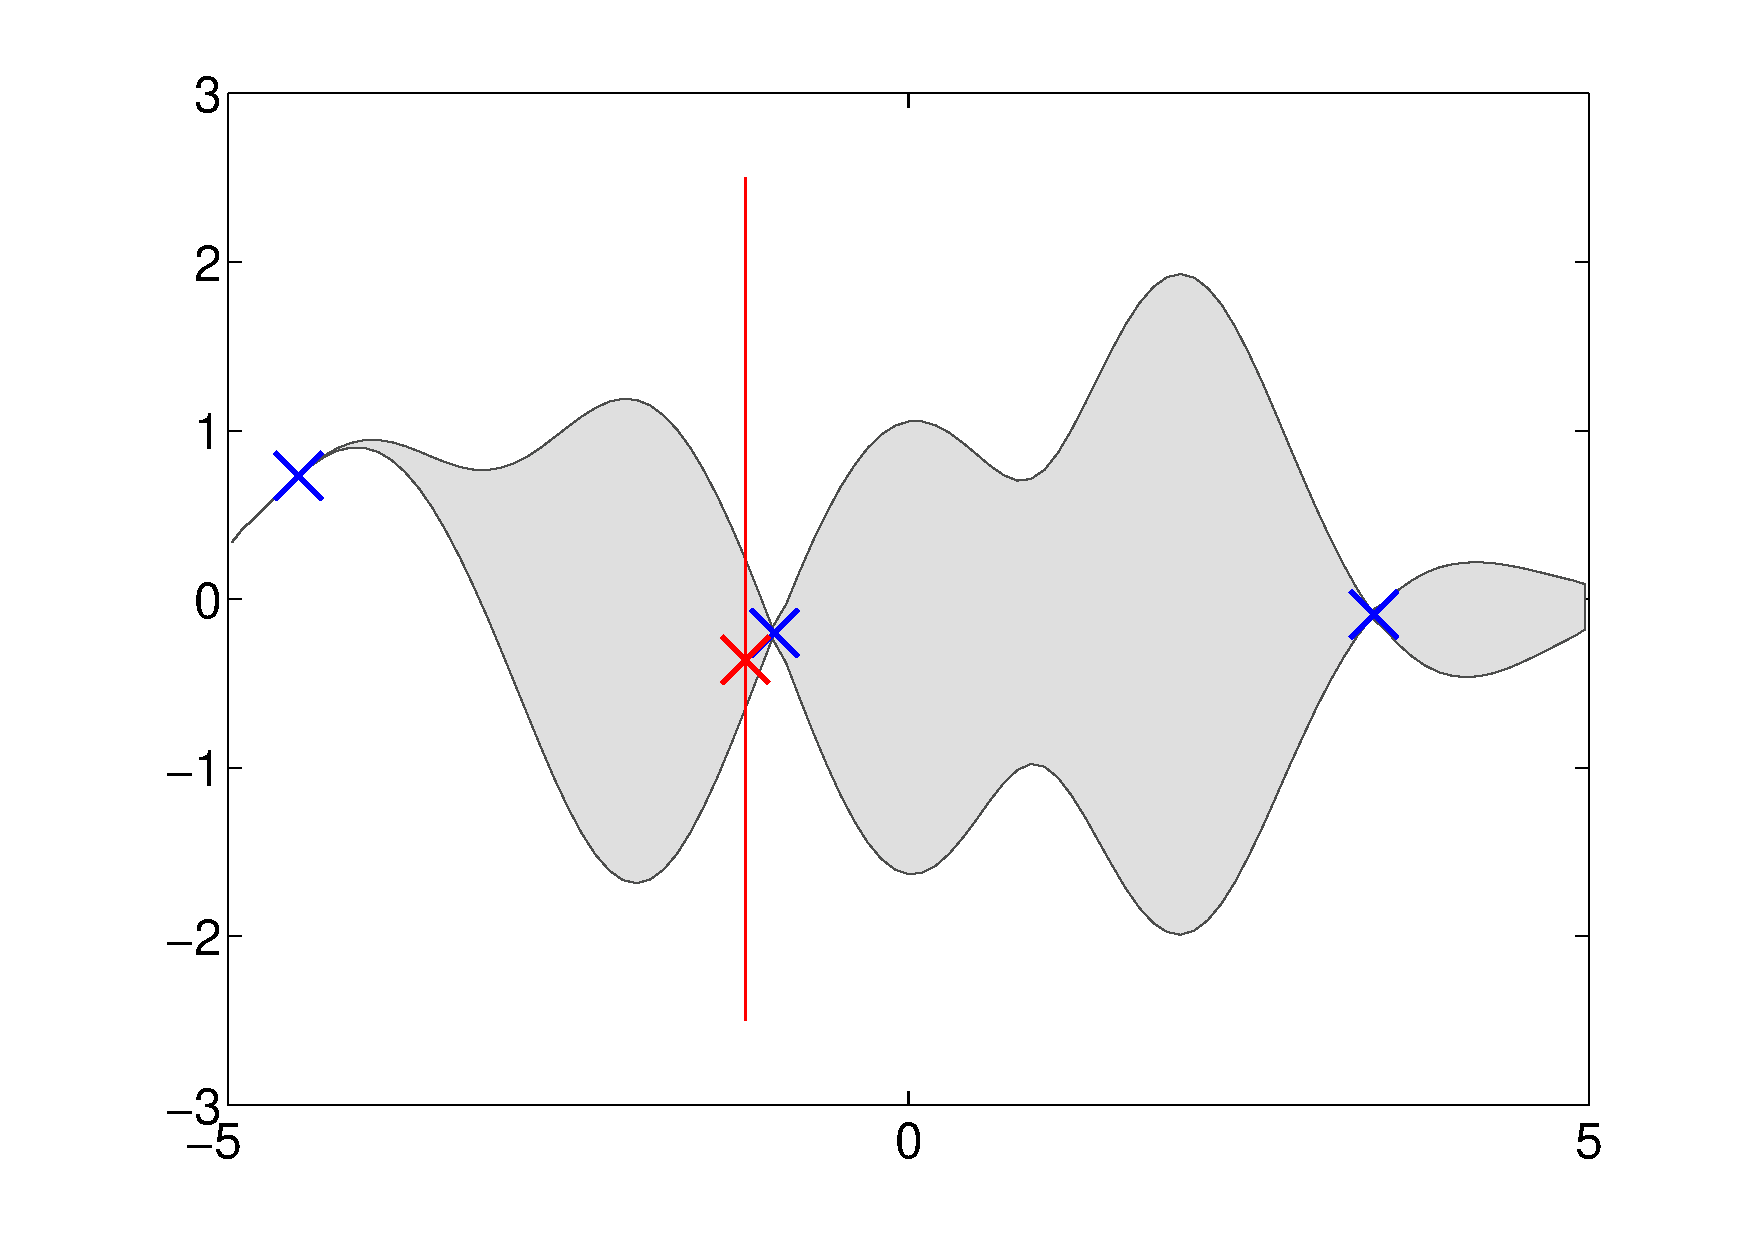
\includegraphics[width=0.33\textwidth]{seq_linear_M4.pdf}
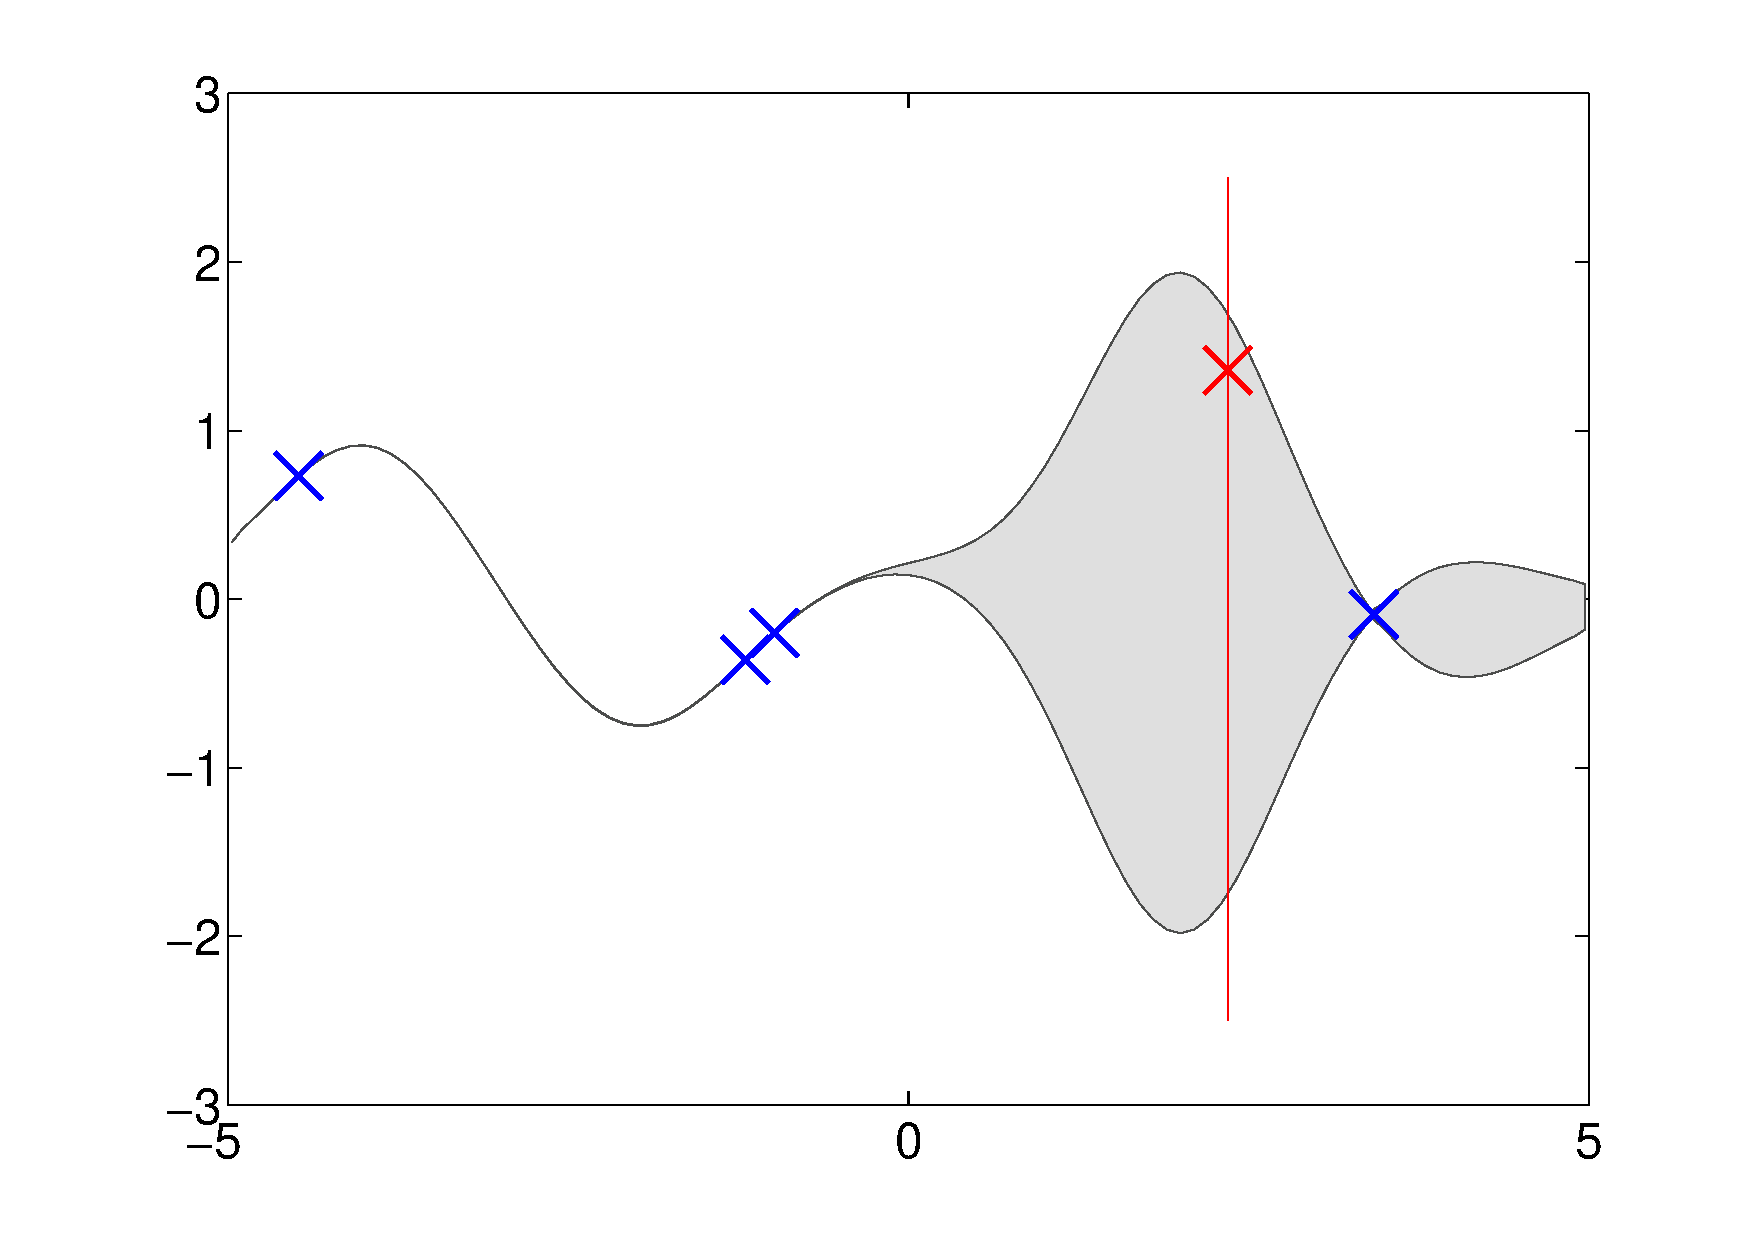
\includegraphics[width=0.33\textwidth]{seq_linear_M5.pdf}
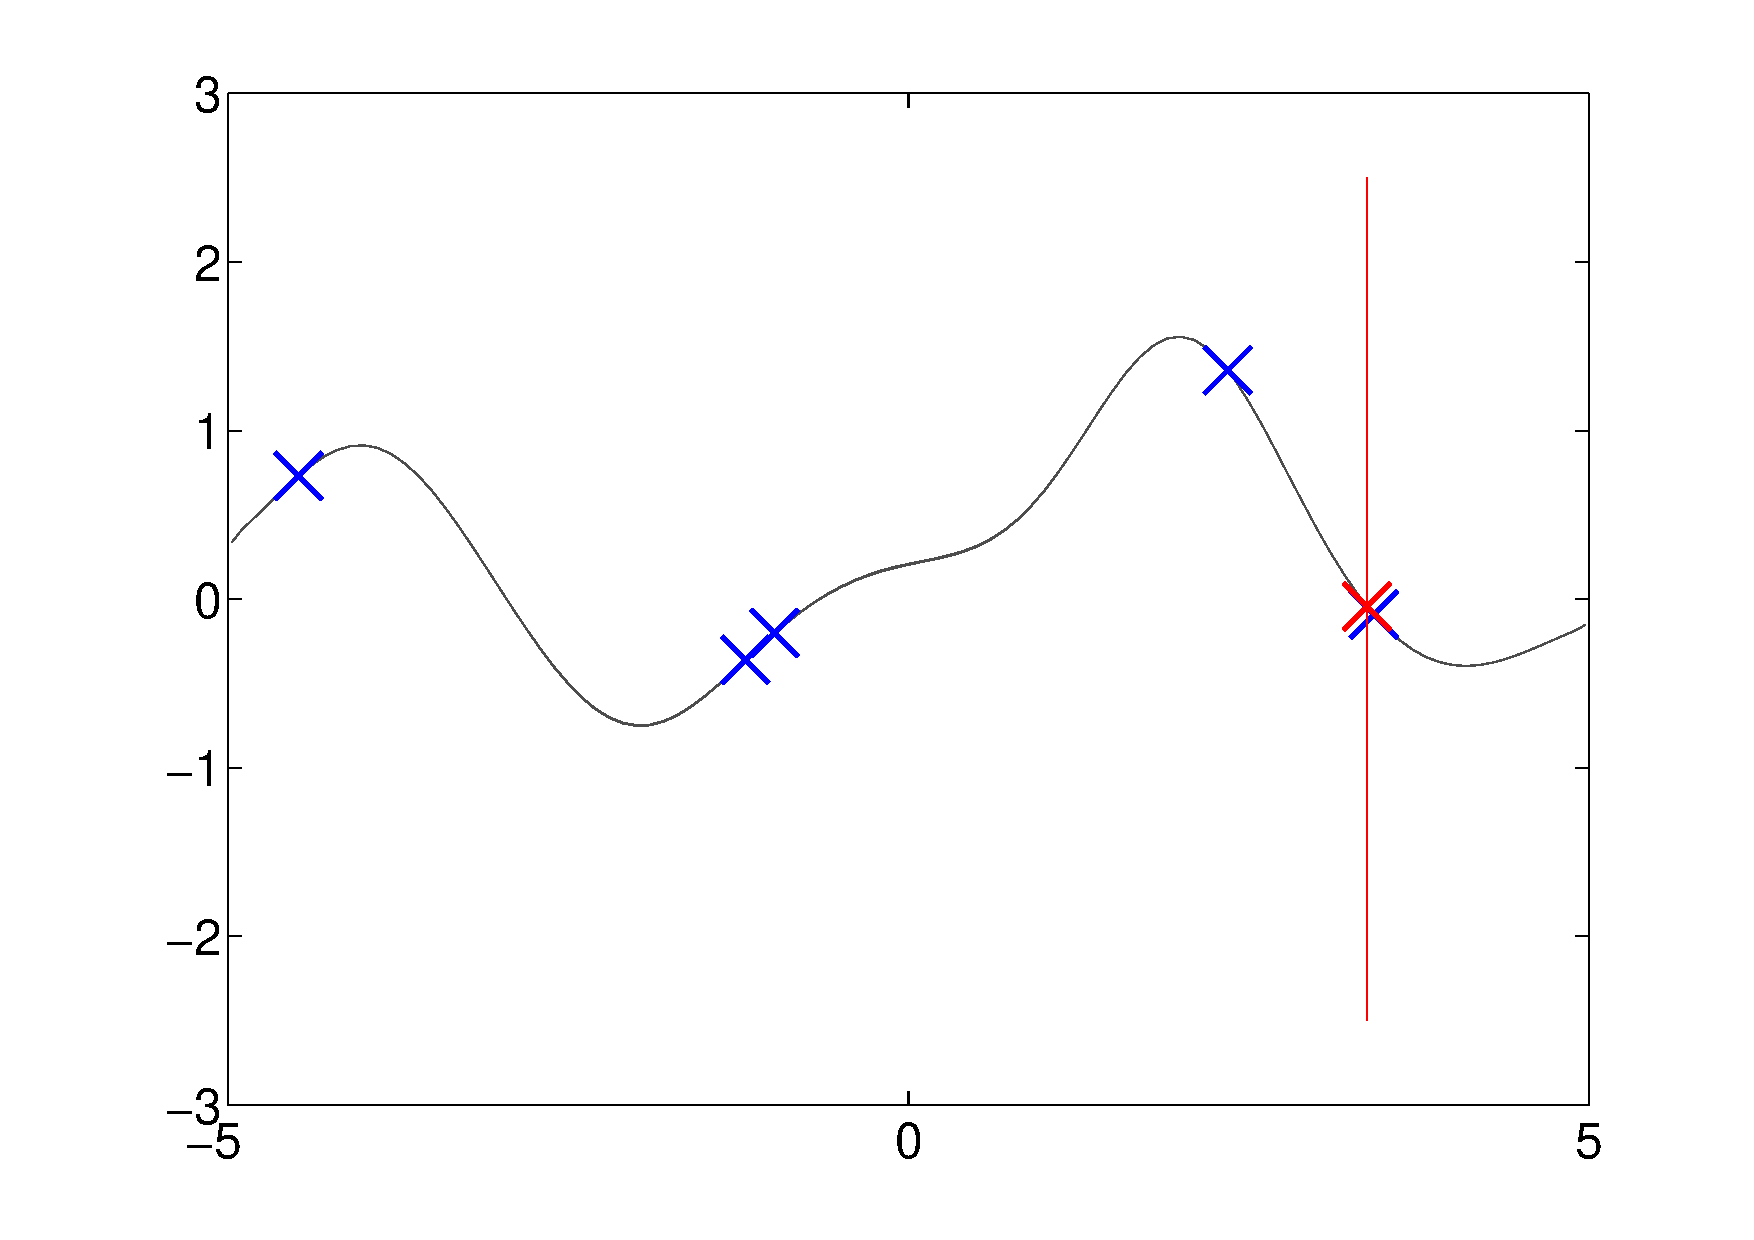
\includegraphics[width=0.33\textwidth]{seq_linear_M6.pdf}

Gaussian process with infinitely many localized basis functions
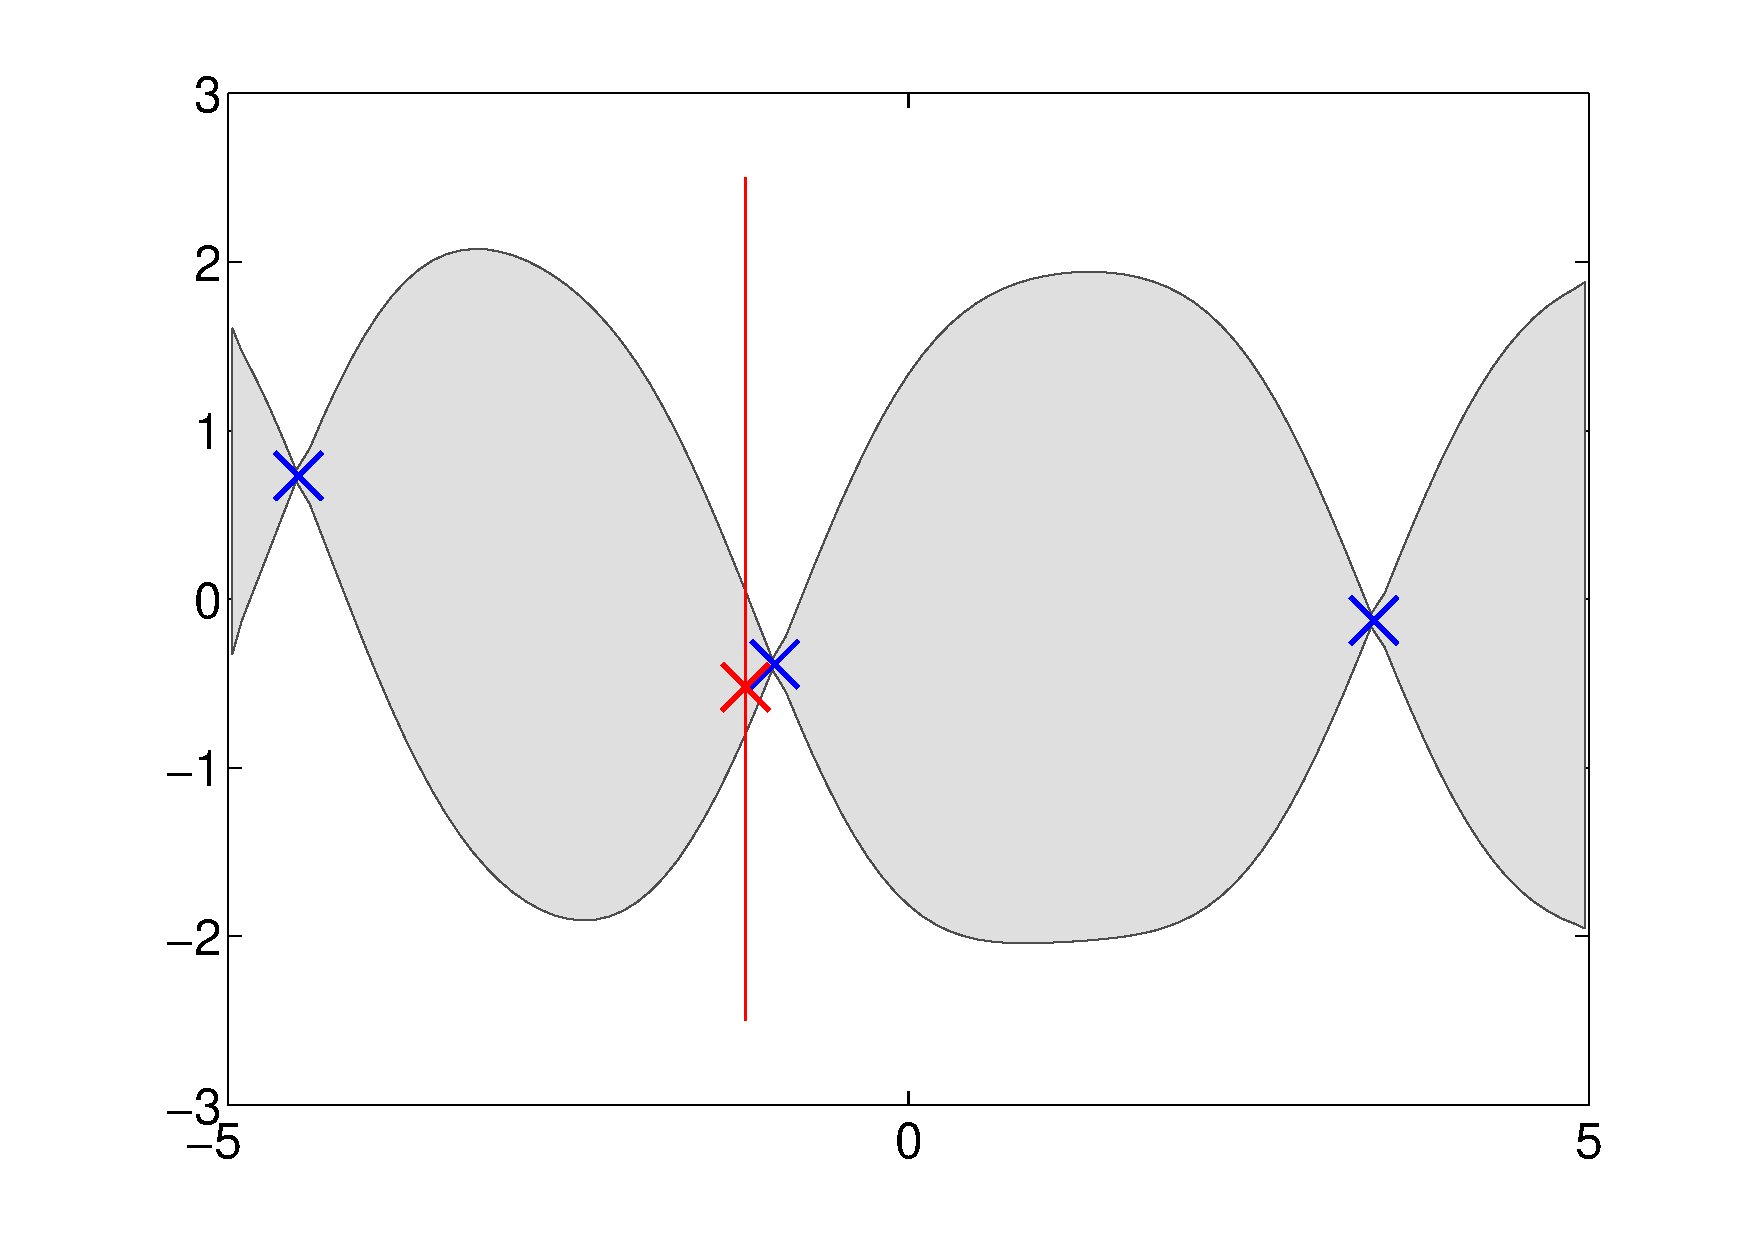
\includegraphics[width=0.33\textwidth]{seq_fullGP_M4.pdf}
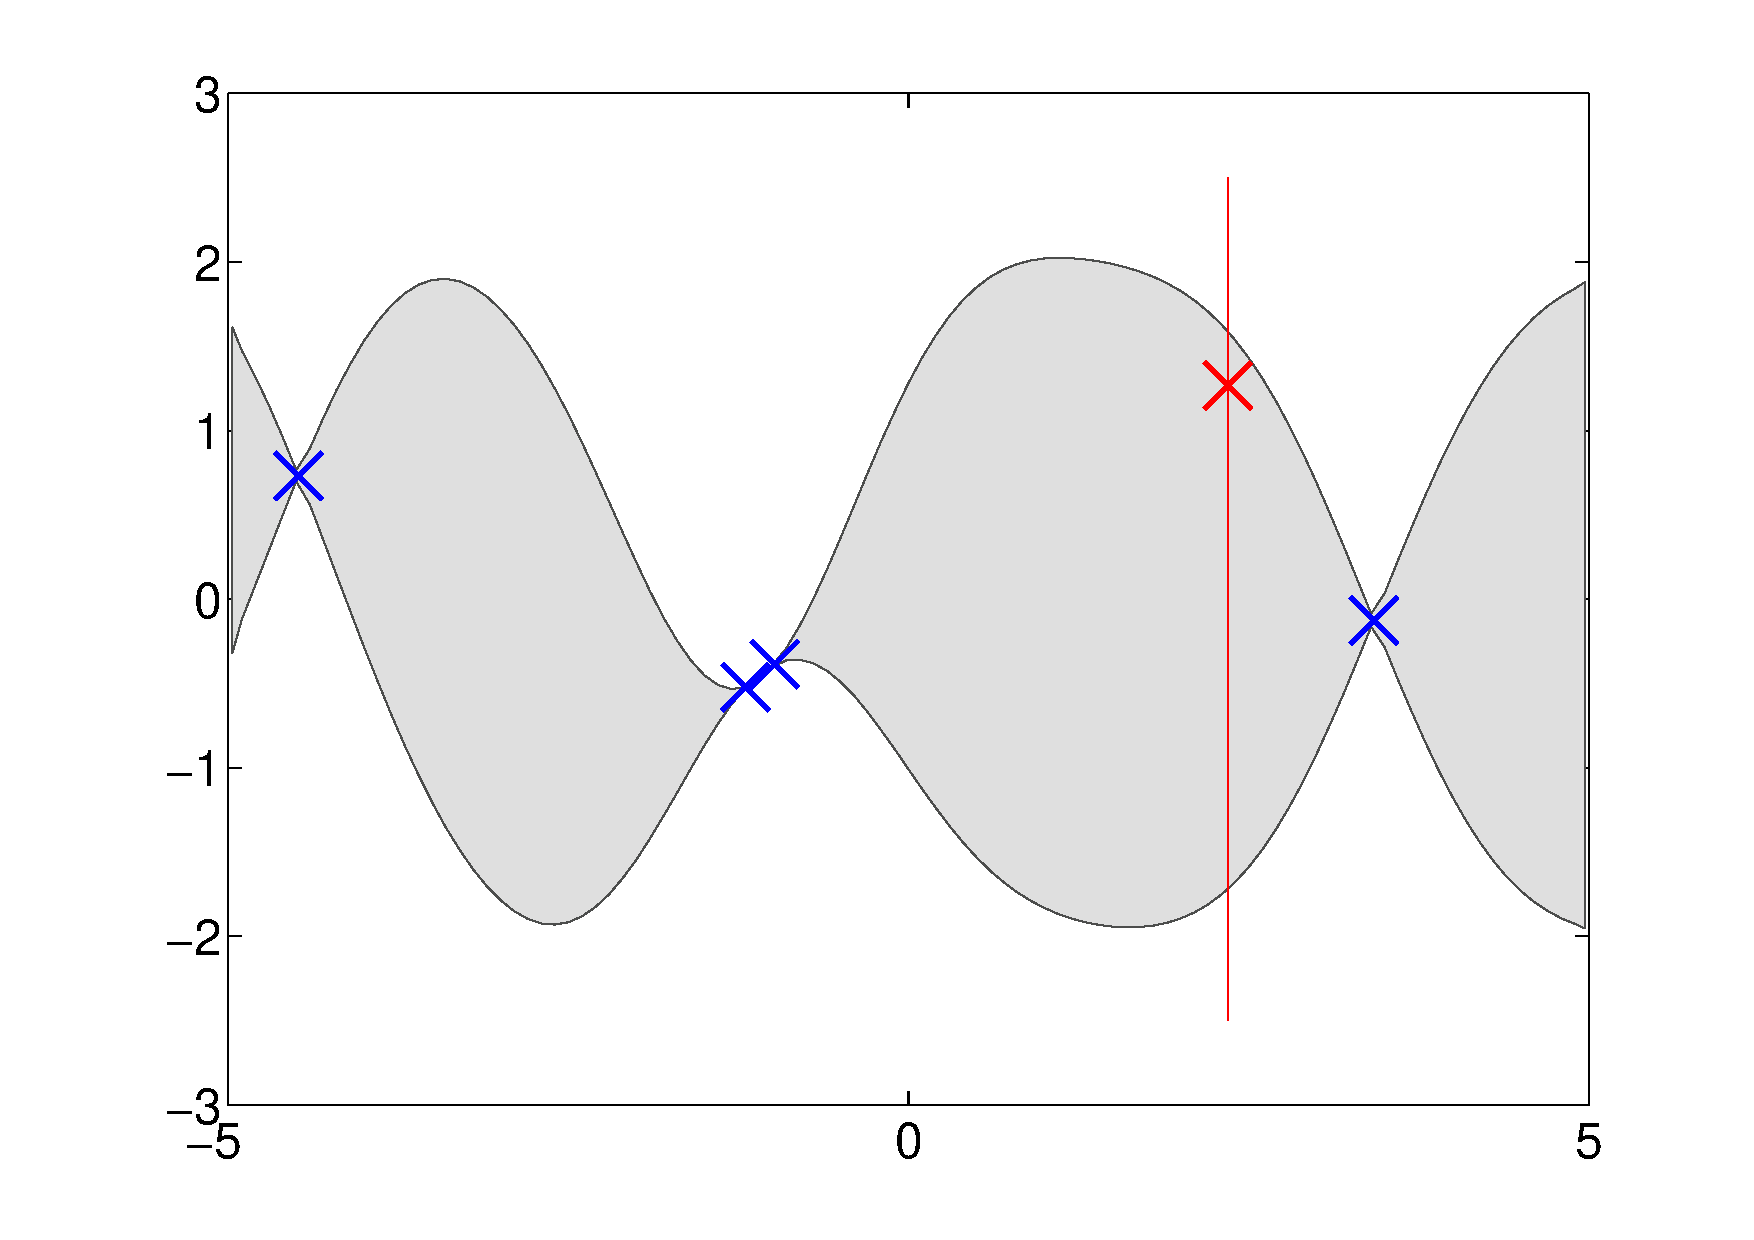
\includegraphics[width=0.33\textwidth]{seq_fullGP_M5.pdf}
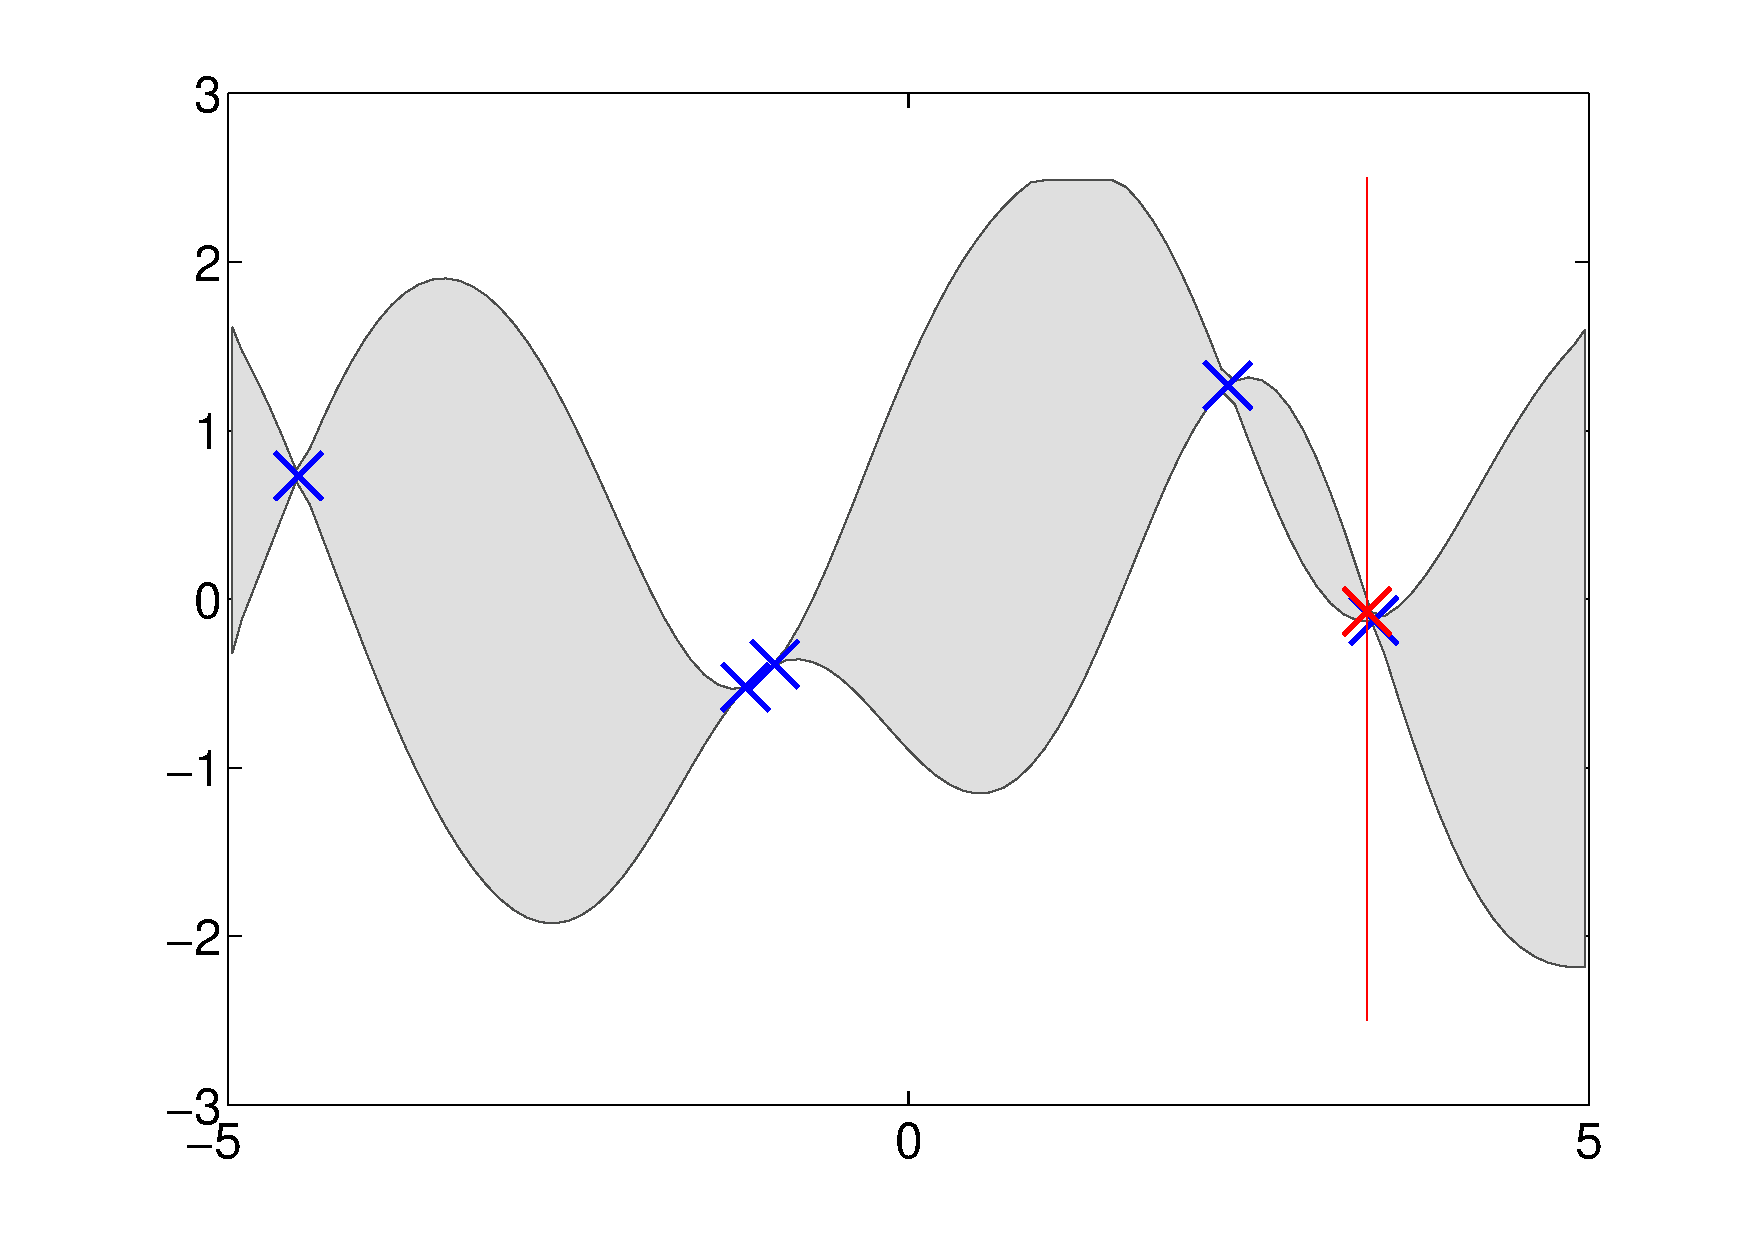
\includegraphics[width=0.33\textwidth]{seq_fullGP_M6.pdf}


\end{frame}


\begin{frame}
\frametitle{\!\!\!Using finitely many basis functions may be dangerous!(3)}


Finite linear model with 5 localized basis functions)

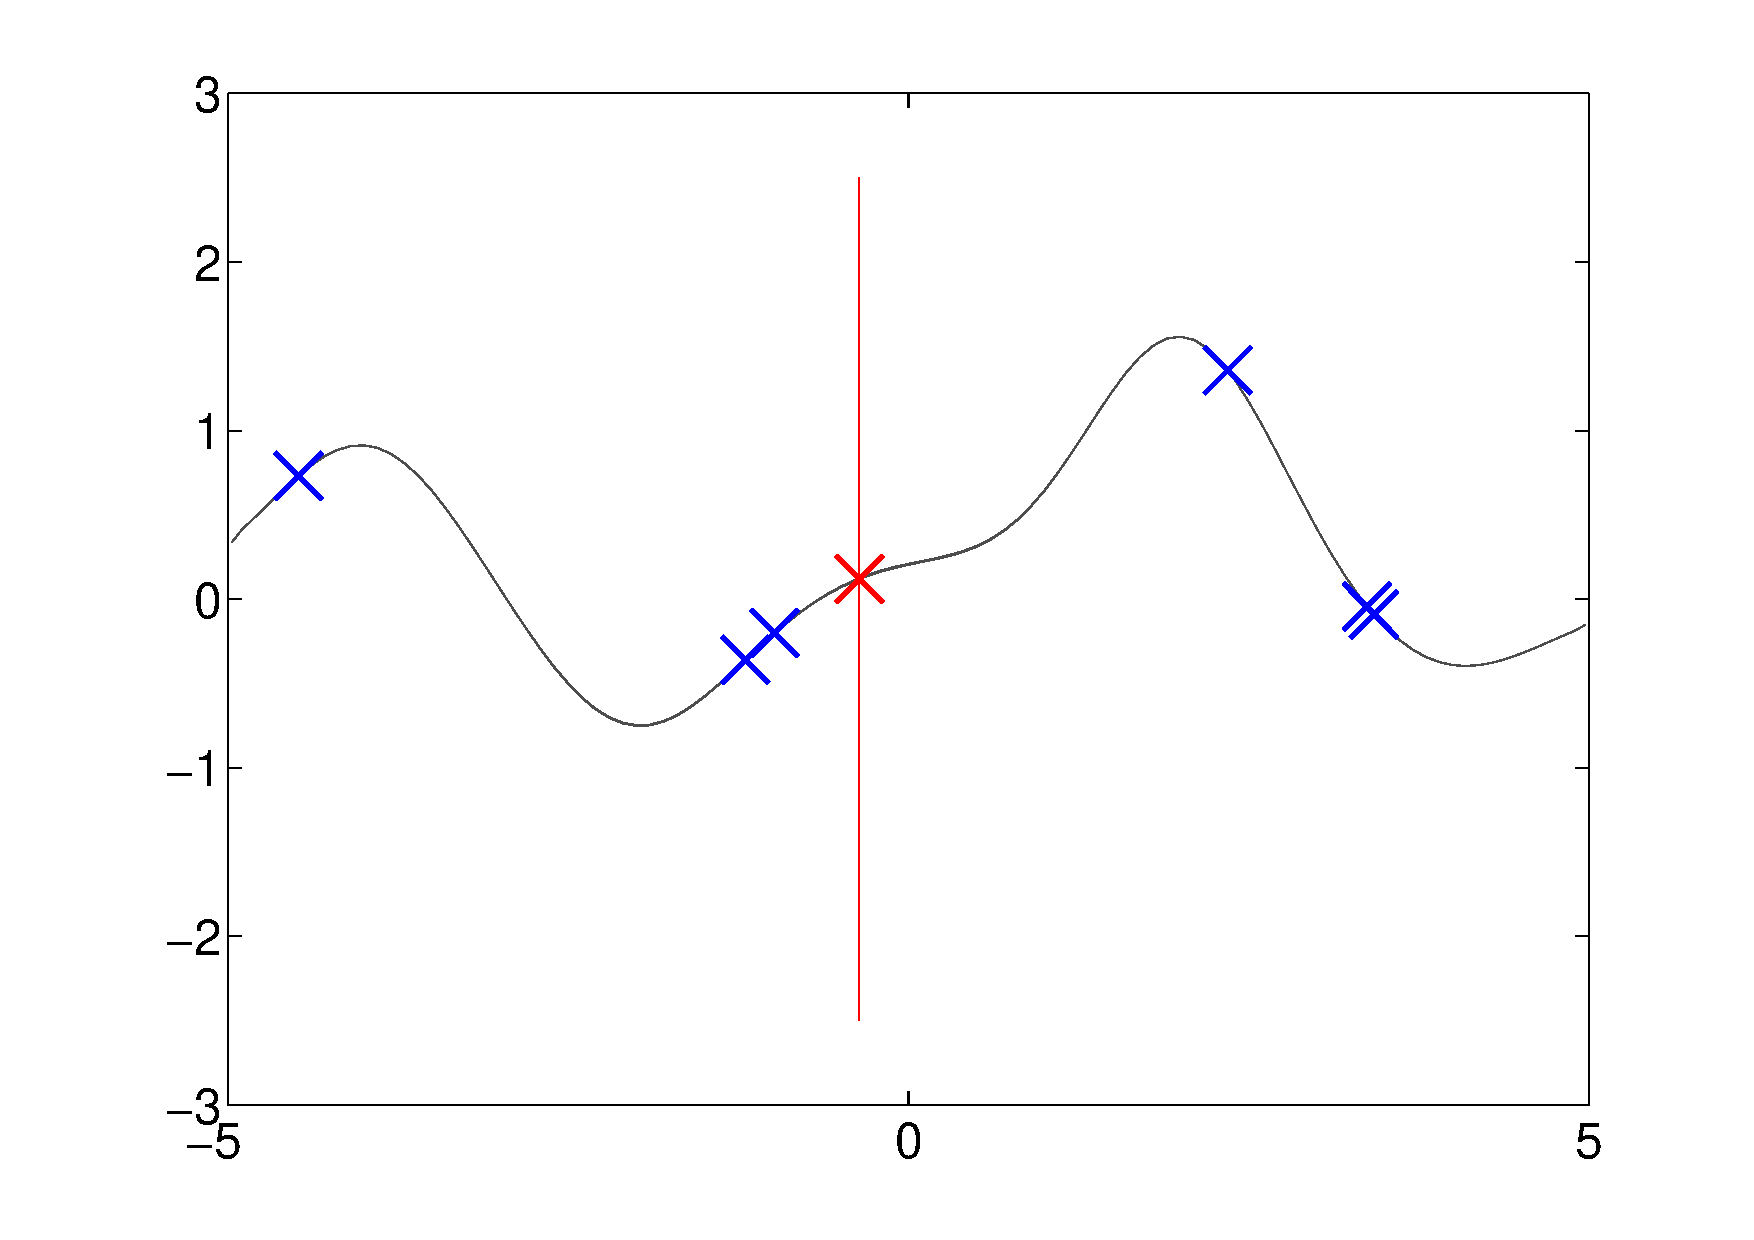
\includegraphics[width=0.33\textwidth]{seq_linear_M7.pdf}
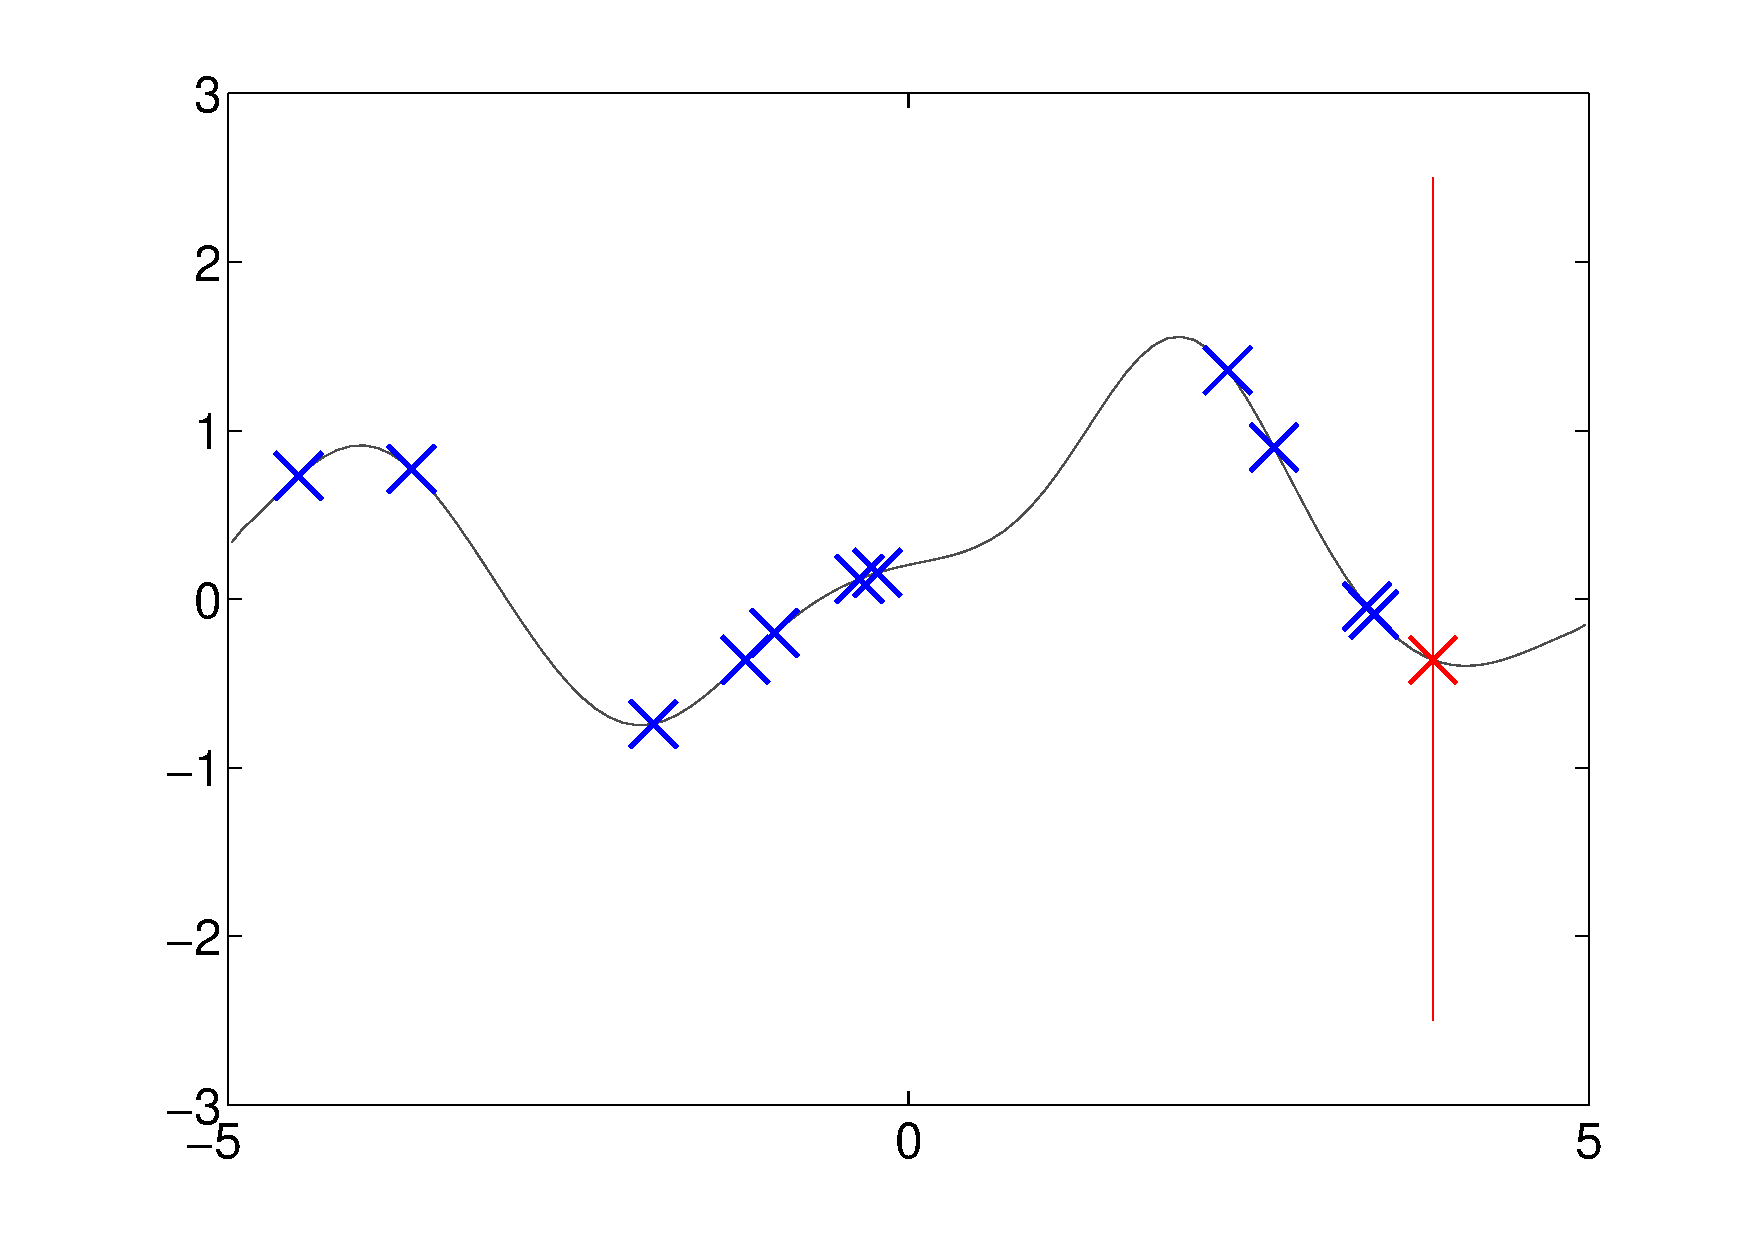
\includegraphics[width=0.33\textwidth]{seq_linear_M12.pdf}
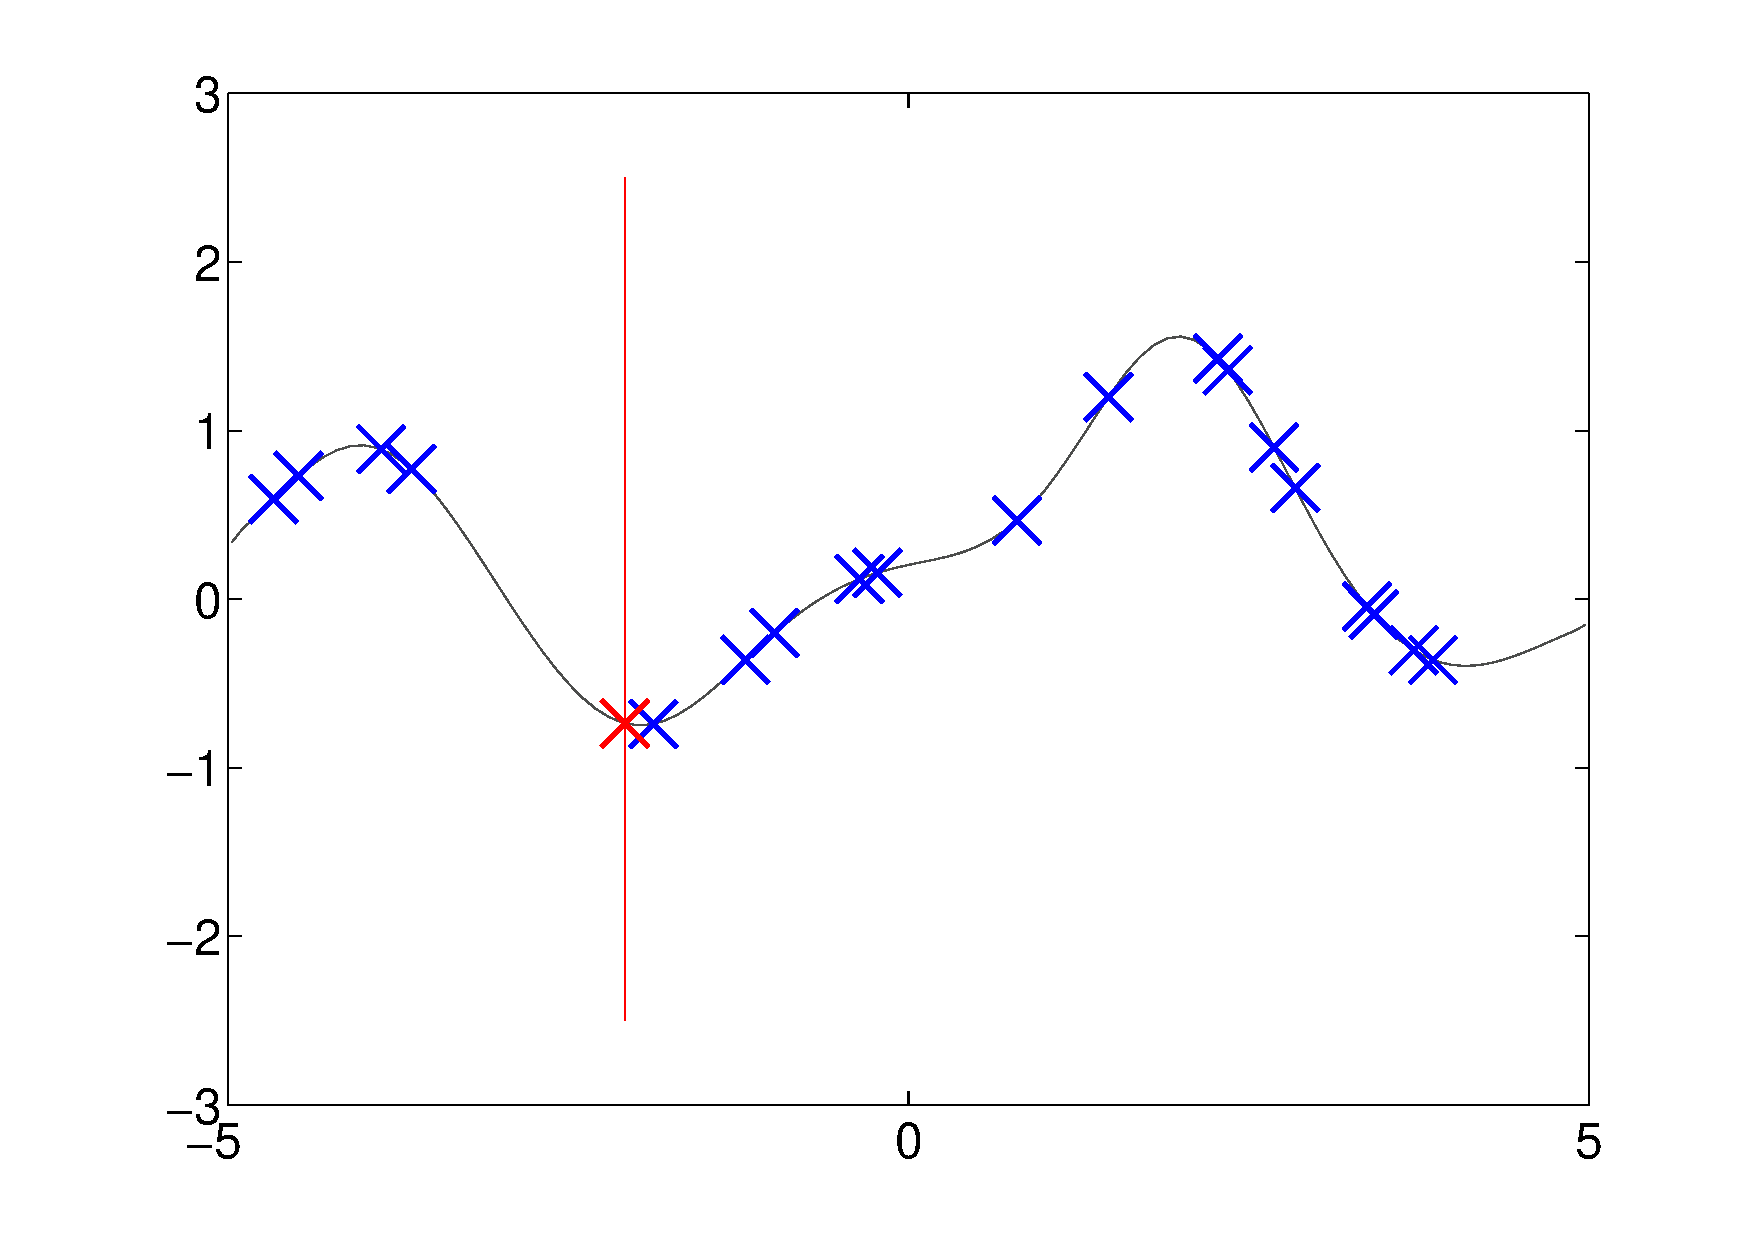
\includegraphics[width=0.33\textwidth]{seq_linear_M20.pdf}

Gaussian process with infinitely many localized basis functions
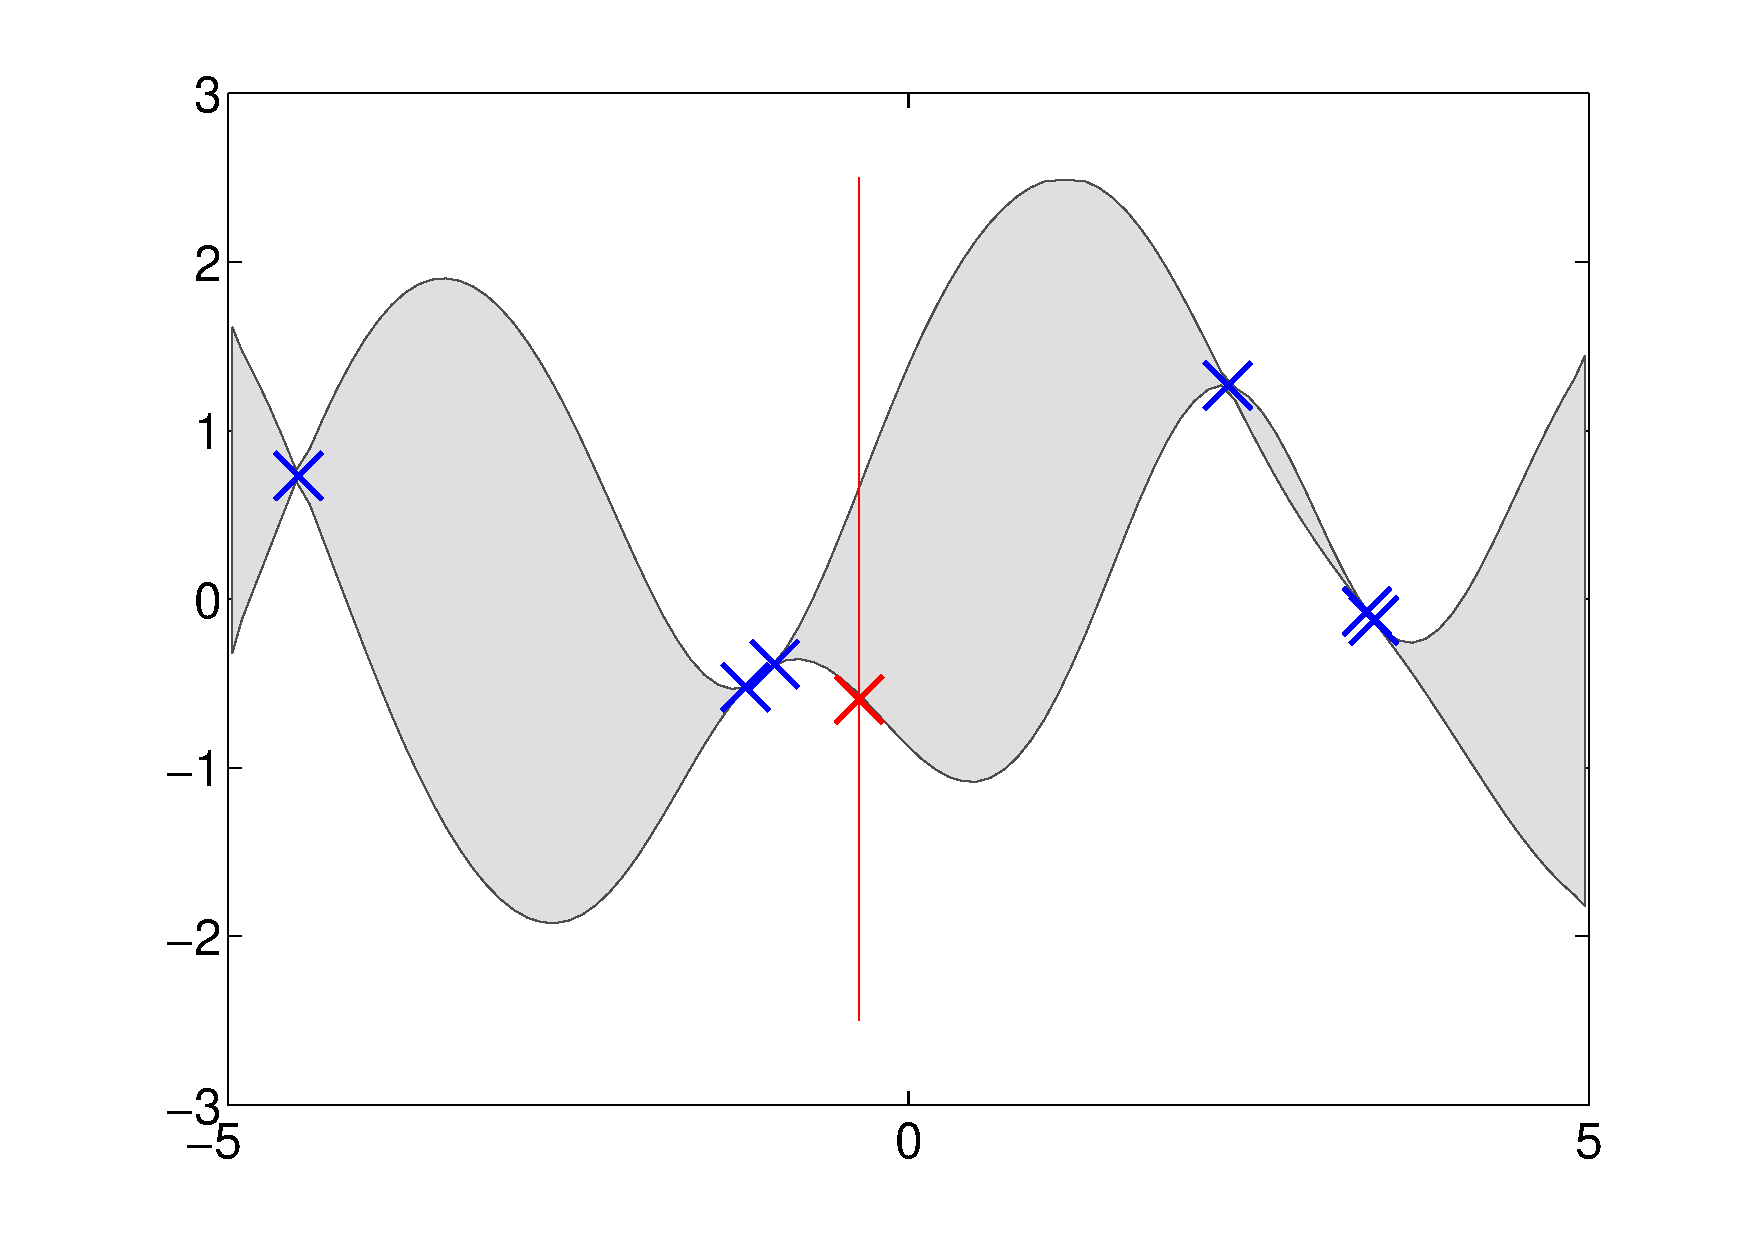
\includegraphics[width=0.33\textwidth]{seq_fullGP_M7.pdf}
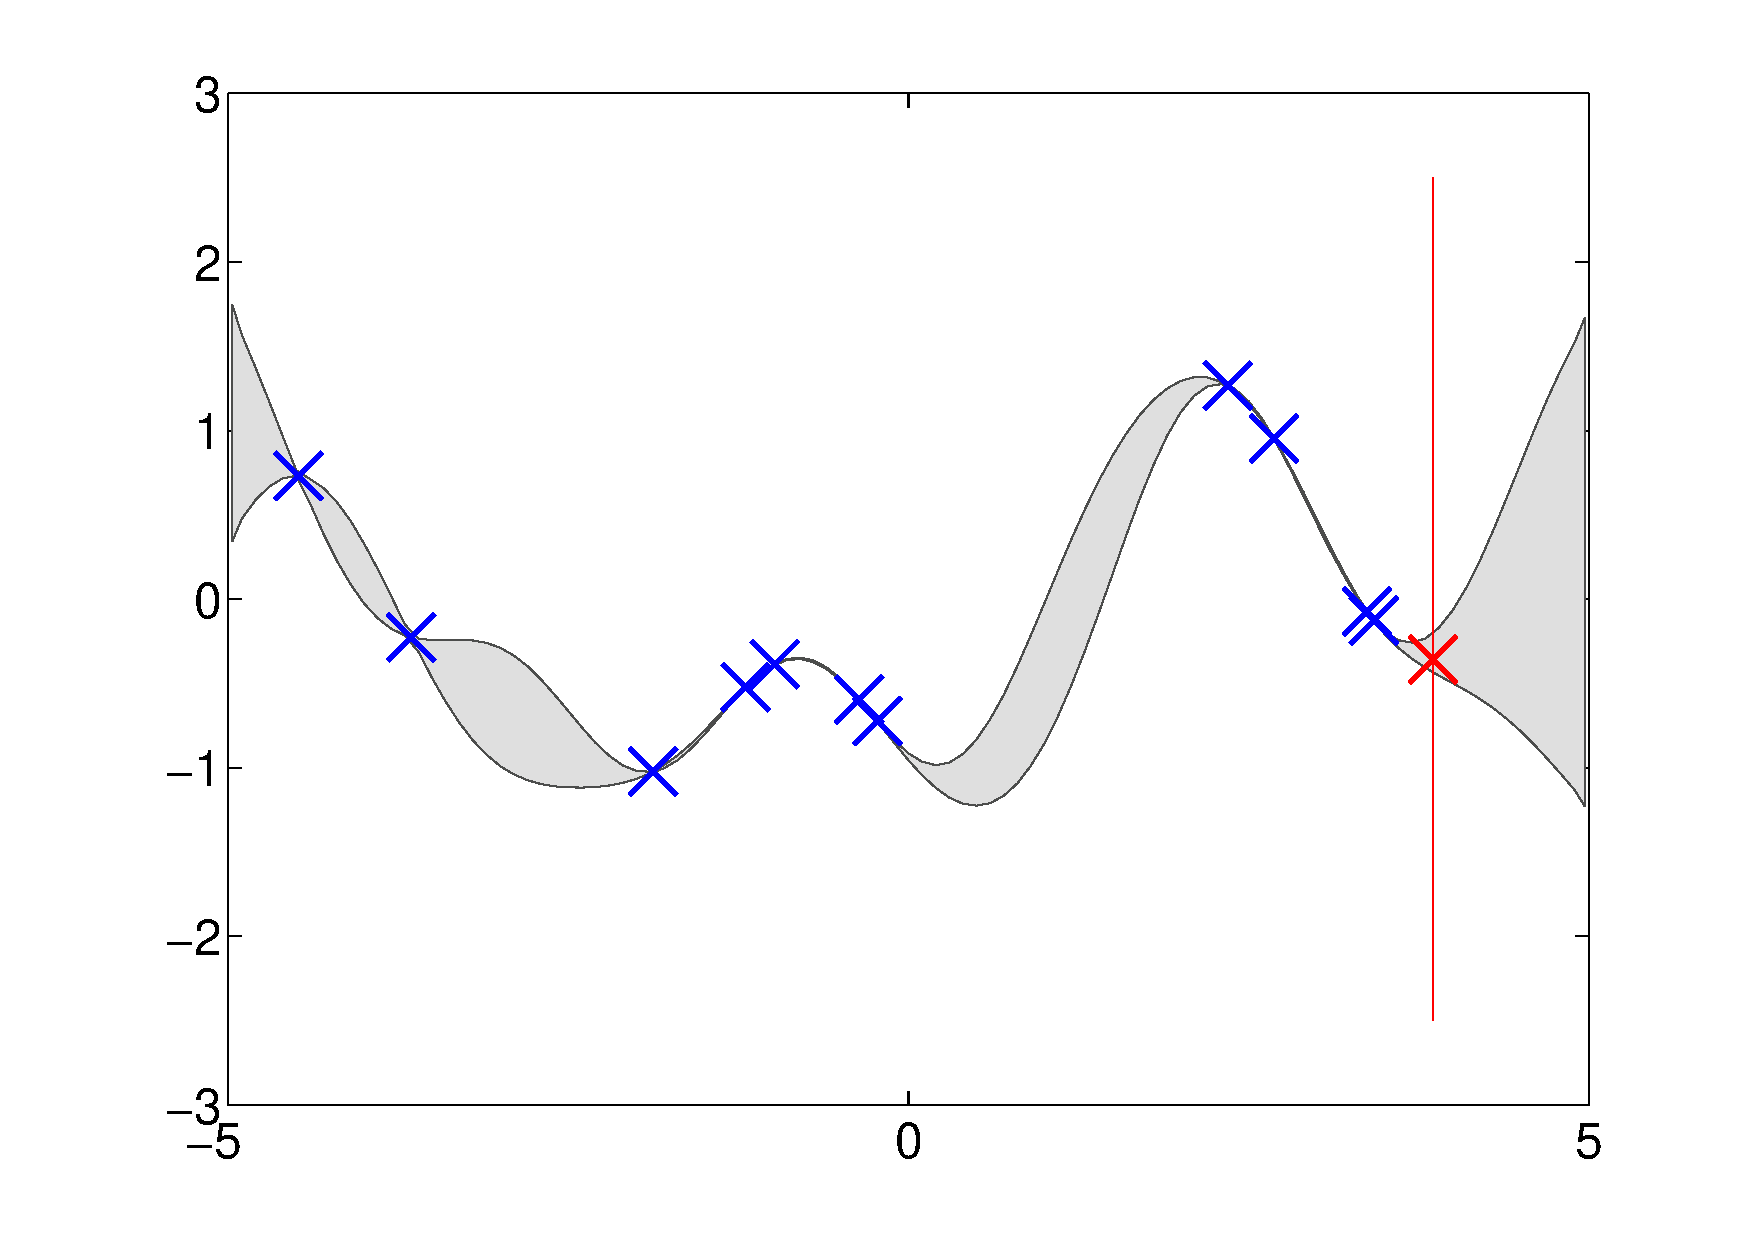
\includegraphics[width=0.33\textwidth]{seq_fullGP_M12.pdf}
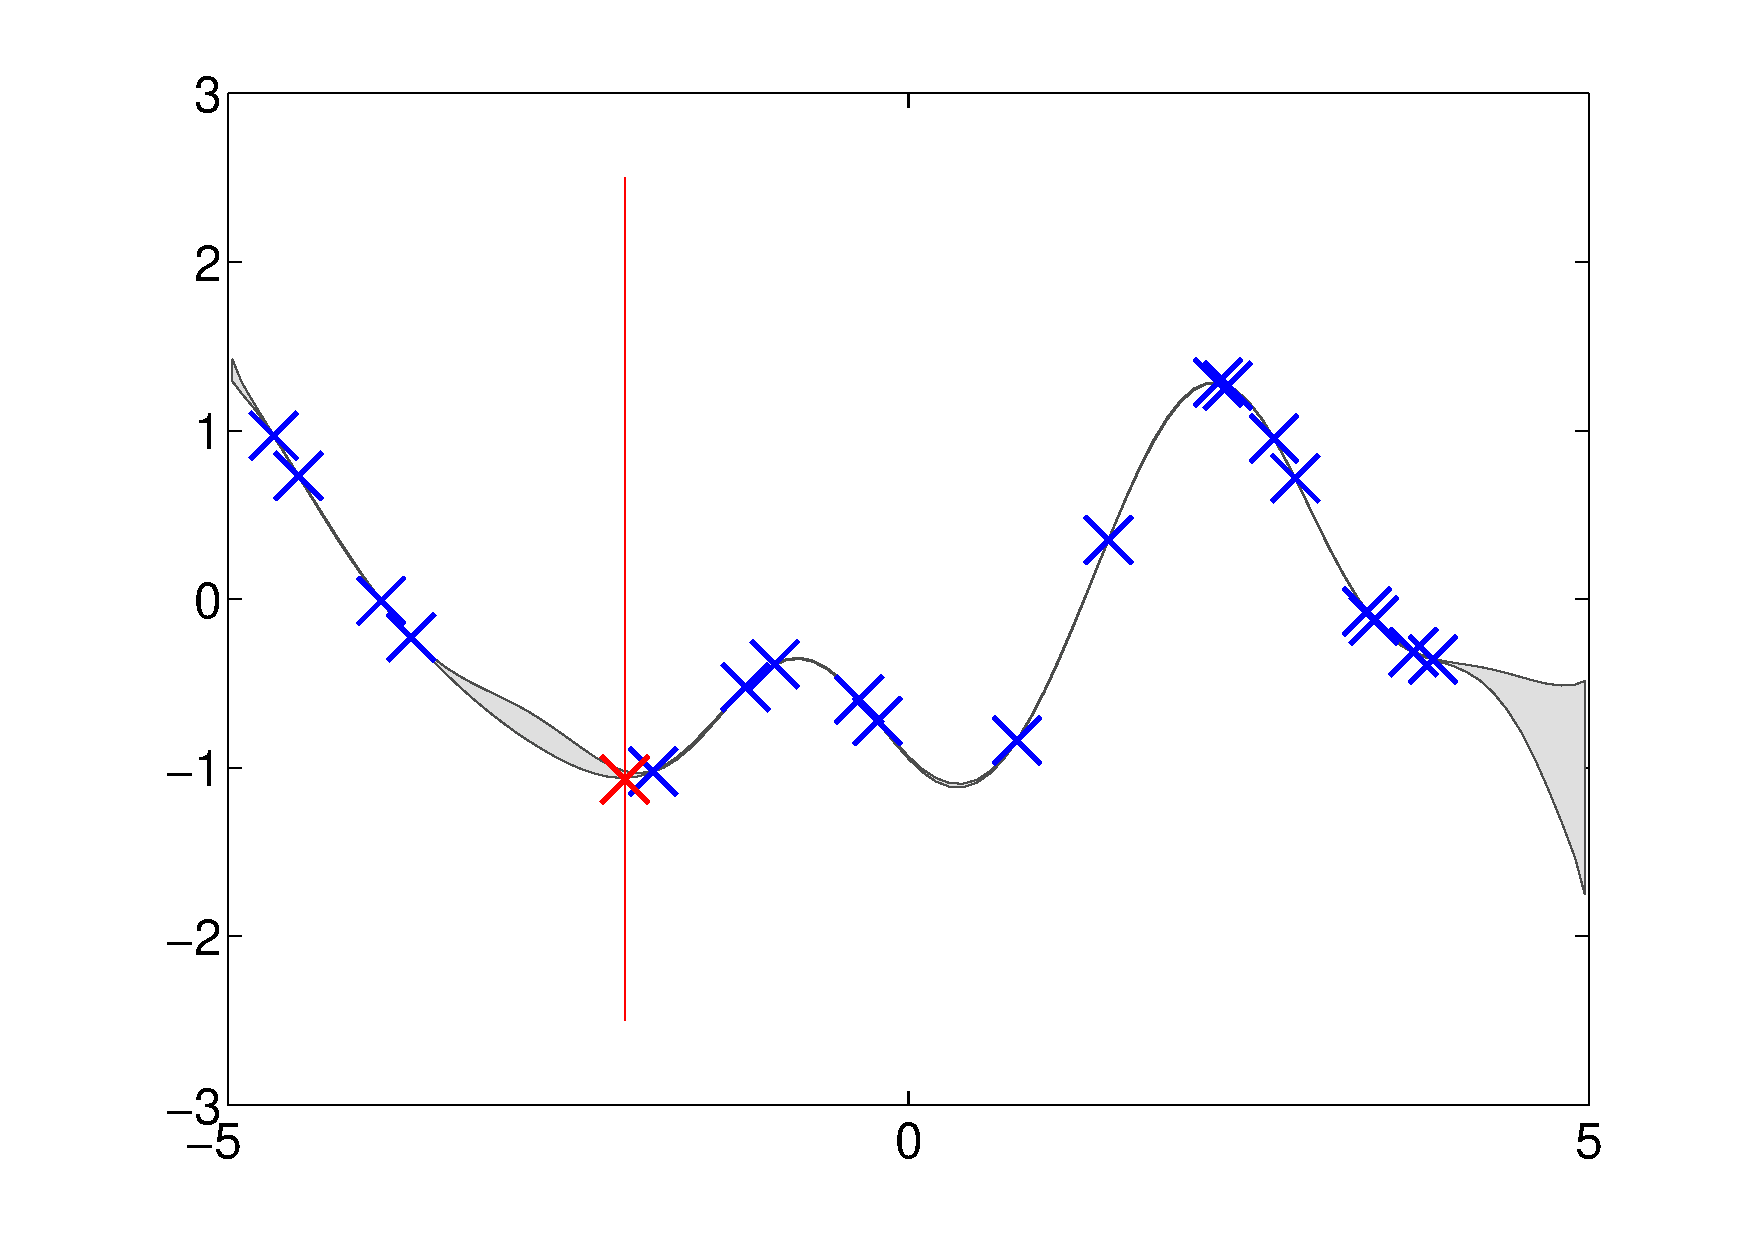
\includegraphics[width=0.33\textwidth]{seq_fullGP_M20.pdf}


\end{frame}


\end{document}
